% ViSongSearch paper draft. Compile: pdflatex main && bibtex main && pdflatex main && pdflatex main
% Numbers and tables in paper/generated/ come from scripts/make_paper_tables.py; regenerate them
% after every experiment instead of editing them by hand.
\documentclass[11pt]{article}
\usepackage{iftex}
\ifXeTeX                            % XeLaTeX/LuaLaTeX: Unicode fonts cover Vietnamese
  \usepackage{fontspec}
\else\ifLuaTeX
  \usepackage{fontspec}
\else                               % pdfLaTeX: Vietnamese letters through vntex (T5)
  \usepackage[T5]{fontenc}
  \usepackage[utf8]{inputenc}
  \usepackage{lmodern}
\fi\fi
\usepackage[a4paper,margin=2.5cm]{geometry}
\usepackage{microtype}
\usepackage{amsmath,amssymb}
\usepackage{booktabs}
\usepackage{graphicx}
\usepackage{xcolor}
\usepackage{enumitem}
\usepackage[numbers,sort&compress]{natbib}
\usepackage[hidelinks]{hyperref}
\usepackage{xspace}

\definecolor{pendingcolor}{HTML}{B3261E}
\newcommand{\pending}[1]{\textcolor{pendingcolor}{\textsf{\small[#1]}}}
\newcommand{\authornote}[1]{\textcolor{blue!55!black}{\textsf{\small[Authors: #1]}}}
\newcommand{\vi}[1]{\textit{#1}}          % Vietnamese example
\newcommand{\gloss}[1]{`#1'}
\newif\ifcoursever\coursevertrue        % course submission (SEG301 + TMG301); set \courseverfalse for the journal
\newcommand{\Qone}{Q1\xspace}
\newcommand{\Qtwo}{Q2\xspace}
\newcommand{\Qthree}{Q3\xspace}
\newcommand{\Qfour}{Q4\xspace}
\newcommand{\Qfive}{Q5\xspace}
\newcommand{\Qfouru}{Q4u\xspace}
\newcommand{\Qfiveu}{Q5u\xspace}
\newcommand{\mrr}{MRR@10\xspace}

% generated by scripts/make_paper_tables.py; do not edit
\newcommand{\ArtistShareFive}{49}
\newcommand{\ArtistShareFiveG}{0}
\newcommand{\ArtistShareFour}{0}
\newcommand{\ArtistShareFourS}{0}
\newcommand{\ArtistShareOne}{0}
\newcommand{\ArtistShareThree}{0}
\newcommand{\ArtistShareThreeU}{0}
\newcommand{\ArtistShareTwo}{0}
\newcommand{\BChar}{1.0}
\newcommand{\BCharFiveX}{0.9}
\newcommand{\BCharFourX}{0.9}
\newcommand{\BMeta}{0.75}
\newcommand{\BNodiac}{1.0}
\newcommand{\BNodiacBi}{0.75}
\newcommand{\BPhon}{0.9}
\newcommand{\BSyl}{1.0}
\newcommand{\BSylBi}{0.9}
\newcommand{\BWord}{1.0}
\newcommand{\BestLexQfour}{0.354}
\newcommand{\BestLexQfourName}{QL Dirichlet, syllables}
\newcommand{\BestLexQfourU}{0.299}
\newcommand{\BestLexQfourUName}{RRF, weights per predicted type}
\newcommand{\BestSingleLexDev}{Restore$_{\mathrm{all}}$ + uni+bigrams}
\newcommand{\BestSingleLexMacro}{0.840}
\newcommand{\CIFuseGlobalHi}{0.855}
\newcommand{\CIFuseGlobalLo}{0.830}
\newcommand{\CIHalfFuseGlobalMax}{0.057}
\newcommand{\CIHalfRestAllBiMax}{0.056}
\newcommand{\CIHalfSelMax}{0.059}
\newcommand{\CIHalfSylMax}{0.054}
\newcommand{\CIRestAllBiHi}{0.853}
\newcommand{\CIRestAllBiLo}{0.827}
\newcommand{\CISelHi}{0.891}
\newcommand{\CISelLo}{0.865}
\newcommand{\CISylHi}{0.537}
\newcommand{\CISylLo}{0.505}
\newcommand{\ChanDiffMaxAbs}{0.042}
\newcommand{\ChanDiffMean}{\ensuremath{+}0.005}
\newcommand{\ChanDiffShareSmall}{87}
\newcommand{\CrawlEnd}{2026-10-31}
\newcommand{\CrawlErrors}{0}
\newcommand{\CrawlIdMax}{90000}
\newcommand{\CrawlPages}{11002}
\newcommand{\CrawlSongs}{8234}
\newcommand{\CrawlStart}{2026-10-31}
\newcommand{\DPMax}{90}
\newcommand{\DPMin}{78}
\newcommand{\DPPairs}{903}
\newcommand{\DPQfive}{78}
\newcommand{\DPQfiveG}{59}
\newcommand{\DPQfiveU}{88}
\newcommand{\DPQfour}{79}
\newcommand{\DPQfourS}{76}
\newcommand{\DPQfourU}{80}
\newcommand{\DPQone}{84}
\newcommand{\DPQthree}{86}
\newcommand{\DPQthreeU}{93}
\newcommand{\DPQtwo}{90}
\newcommand{\DefWFinal}{15}
\newcommand{\DefWInitial}{30}
\newcommand{\DefWTone}{25}
\newcommand{\DefWTypo}{30}
\newcommand{\EffEncodeMinBkai}{45}
\newcommand{\EffEncodeMinEbase}{47}
\newcommand{\EffEncodeMinEsmall}{16}
\newcommand{\EffEncodeMinNaftesmalls}{13}
\newcommand{\EffHybridMs}{11}
\newcommand{\EffIndexMBBkai}{244}
\newcommand{\EffIndexMBEbase}{244}
\newcommand{\EffIndexMBEsmall}{122}
\newcommand{\EffIndexMBNaftesmalls}{122}
\newcommand{\EffLexIndexSNodiac}{4}
\newcommand{\EffLexIndexSSyl}{3}
\newcommand{\EffLexMsNodiac}{0.4}
\newcommand{\EffLexMsSyl}{0.3}
\newcommand{\EffPassPerSecBkai}{29}
\newcommand{\EffPassPerSecEbase}{28}
\newcommand{\EffPassPerSecEsmall}{83}
\newcommand{\EffPassPerSecNaftesmalls}{99}
\newcommand{\EffQueryMsBkai}{14}
\newcommand{\EffQueryMsEbase}{15}
\newcommand{\EffQueryMsEsmall}{6}
\newcommand{\EffQueryMsNaftesmalls}{5}
\newcommand{\EffSearchMsBkai}{8}
\newcommand{\EffSearchMsEbase}{9}
\newcommand{\EffSearchMsEsmall}{5}
\newcommand{\EffSearchMsNaftesmalls}{5}
\newcommand{\FormsPerUnmarked}{8.0}
\newcommand{\FuseGlobalWeights}{(2, 0.5, 0, 0)}
\newcommand{\FuseQfourCvGlobal}{0.340}
\newcommand{\FuseQfourCvType}{0.356}
\newcommand{\FuseQfourWeights}{(1, 0, 0, 0)}
\newcommand{\FuseQthreeCvGlobal}{0.938}
\newcommand{\FuseQthreeCvType}{0.950}
\newcommand{\FuseQthreeWeights}{(0.5, 2, 0, 0)}
\newcommand{\FuseTrainTypesKept}{Q2, Q3, Q4, Q4u, Q5, Q5u}
\newcommand{\FuseTypesKept}{Q3, Q4}
\newcommand{\KoneChar}{0.6}
\newcommand{\KoneCharFiveX}{0.6}
\newcommand{\KoneCharFourX}{0.6}
\newcommand{\KoneMeta}{0.9}
\newcommand{\KoneNodiac}{0.6}
\newcommand{\KoneNodiacBi}{0.3}
\newcommand{\KonePhon}{0.3}
\newcommand{\KoneSyl}{0.3}
\newcommand{\KoneSylBi}{0.3}
\newcommand{\KoneWord}{0.3}
\newcommand{\LSHBands}{42}
\newcommand{\LSHRows}{3}
\newcommand{\LargestCluster}{9}
\newcommand{\LenFive}{27.2}
\newcommand{\LenFiveG}{25.0}
\newcommand{\LenFour}{17.2}
\newcommand{\LenFourS}{10.7}
\newcommand{\LenOne}{8.5}
\newcommand{\LenThree}{8.5}
\newcommand{\LenThreeU}{8.5}
\newcommand{\LenTwo}{8.5}
\newcommand{\LexRefName}{RRF, weights tuned on dev}
\newcommand{\MCharEFifty}{0.113}
\newcommand{\MCharEForty}{0.154}
\newcommand{\MCharETen}{0.383}
\newcommand{\MCharEThirty}{0.209}
\newcommand{\MCharETwenty}{0.297}
\newcommand{\MCharFive}{0.443}
\newcommand{\MCharFiveG}{0.096}
\newcommand{\MCharFiveU}{0.443}
\newcommand{\MCharFiveXEFifty}{0.857}
\newcommand{\MCharFiveXEForty}{0.908}
\newcommand{\MCharFiveXETen}{0.970}
\newcommand{\MCharFiveXEThirty}{0.937}
\newcommand{\MCharFiveXETwenty}{0.966}
\newcommand{\MCharFiveXFive}{0.840}
\newcommand{\MCharFiveXFiveG}{0.190}
\newcommand{\MCharFiveXFiveU}{0.840}
\newcommand{\MCharFiveXFour}{0.248}
\newcommand{\MCharFiveXFourS}{0.118}
\newcommand{\MCharFiveXFourU}{0.248}
\newcommand{\MCharFiveXMacro}{0.801}
\newcommand{\MCharFiveXNFifty}{0.844}
\newcommand{\MCharFiveXNForty}{0.907}
\newcommand{\MCharFiveXNTen}{0.965}
\newcommand{\MCharFiveXNThirty}{0.916}
\newcommand{\MCharFiveXNTwenty}{0.968}
\newcommand{\MCharFiveXNZero}{0.989}
\newcommand{\MCharFiveXOne}{0.989}
\newcommand{\MCharFiveXThree}{0.941}
\newcommand{\MCharFiveXThreeU}{0.933}
\newcommand{\MCharFiveXTwo}{0.985}
\newcommand{\MCharFiveXWFifty}{0.673}
\newcommand{\MCharFiveXWForty}{0.829}
\newcommand{\MCharFiveXWTen}{0.942}
\newcommand{\MCharFiveXWThirty}{0.856}
\newcommand{\MCharFiveXWTwenty}{0.930}
\newcommand{\MCharFour}{0.157}
\newcommand{\MCharFourS}{0.079}
\newcommand{\MCharFourU}{0.157}
\newcommand{\MCharFourXEFifty}{0.679}
\newcommand{\MCharFourXEForty}{0.759}
\newcommand{\MCharFourXETen}{0.901}
\newcommand{\MCharFourXEThirty}{0.816}
\newcommand{\MCharFourXETwenty}{0.878}
\newcommand{\MCharFourXFive}{0.677}
\newcommand{\MCharFourXFiveG}{0.121}
\newcommand{\MCharFourXFiveU}{0.677}
\newcommand{\MCharFourXFour}{0.196}
\newcommand{\MCharFourXFourS}{0.090}
\newcommand{\MCharFourXFourU}{0.196}
\newcommand{\MCharFourXMacro}{0.717}
\newcommand{\MCharFourXNFifty}{0.639}
\newcommand{\MCharFourXNForty}{0.730}
\newcommand{\MCharFourXNTen}{0.891}
\newcommand{\MCharFourXNThirty}{0.795}
\newcommand{\MCharFourXNTwenty}{0.873}
\newcommand{\MCharFourXNZero}{0.955}
\newcommand{\MCharFourXOne}{0.955}
\newcommand{\MCharFourXThree}{0.811}
\newcommand{\MCharFourXThreeU}{0.795}
\newcommand{\MCharFourXTwo}{0.944}
\newcommand{\MCharFourXWFifty}{0.473}
\newcommand{\MCharFourXWForty}{0.628}
\newcommand{\MCharFourXWTen}{0.858}
\newcommand{\MCharFourXWThirty}{0.718}
\newcommand{\MCharFourXWTwenty}{0.831}
\newcommand{\MCharMacro}{0.410}
\newcommand{\MCharNFifty}{0.118}
\newcommand{\MCharNForty}{0.151}
\newcommand{\MCharNTen}{0.396}
\newcommand{\MCharNThirty}{0.218}
\newcommand{\MCharNTwenty}{0.307}
\newcommand{\MCharNZero}{0.616}
\newcommand{\MCharOne}{0.616}
\newcommand{\MCharThree}{0.270}
\newcommand{\MCharThreeU}{0.253}
\newcommand{\MCharTwo}{0.566}
\newcommand{\MCharWFifty}{0.155}
\newcommand{\MCharWForty}{0.218}
\newcommand{\MCharWTen}{0.459}
\newcommand{\MCharWThirty}{0.283}
\newcommand{\MCharWTwenty}{0.394}
\newcommand{\MFirstSampleFive}{0.928}
\newcommand{\MFirstSampleFiveG}{0.242}
\newcommand{\MFirstSampleFiveU}{0.911}
\newcommand{\MFirstSampleFour}{0.532}
\newcommand{\MFirstSampleFourS}{0.195}
\newcommand{\MFirstSampleFourU}{0.518}
\newcommand{\MFirstSampleMacro}{0.880}
\newcommand{\MFirstSampleOne}{0.993}
\newcommand{\MFirstSampleThree}{0.949}
\newcommand{\MFirstSampleThreeU}{0.885}
\newcommand{\MFirstSampleTwo}{0.996}
\newcommand{\MFuseAdaptiveEFifty}{0.769}
\newcommand{\MFuseAdaptiveEForty}{0.875}
\newcommand{\MFuseAdaptiveETen}{0.984}
\newcommand{\MFuseAdaptiveEThirty}{0.931}
\newcommand{\MFuseAdaptiveETwenty}{0.976}
\newcommand{\MFuseAdaptiveFive}{0.930}
\newcommand{\MFuseAdaptiveFiveG}{0.242}
\newcommand{\MFuseAdaptiveFiveU}{0.910}
\newcommand{\MFuseAdaptiveFour}{0.336}
\newcommand{\MFuseAdaptiveFourS}{0.194}
\newcommand{\MFuseAdaptiveFourU}{0.299}
\newcommand{\MFuseAdaptiveMacro}{0.840}
\newcommand{\MFuseAdaptiveNFifty}{0.758}
\newcommand{\MFuseAdaptiveNForty}{0.875}
\newcommand{\MFuseAdaptiveNTen}{0.981}
\newcommand{\MFuseAdaptiveNThirty}{0.906}
\newcommand{\MFuseAdaptiveNTwenty}{0.979}
\newcommand{\MFuseAdaptiveNZero}{0.999}
\newcommand{\MFuseAdaptiveOne}{0.999}
\newcommand{\MFuseAdaptiveThree}{0.943}
\newcommand{\MFuseAdaptiveThreeU}{0.893}
\newcommand{\MFuseAdaptiveTwo}{0.995}
\newcommand{\MFuseAdaptiveWFifty}{0.726}
\newcommand{\MFuseAdaptiveWForty}{0.877}
\newcommand{\MFuseAdaptiveWTen}{0.979}
\newcommand{\MFuseAdaptiveWThirty}{0.909}
\newcommand{\MFuseAdaptiveWTwenty}{0.980}
\newcommand{\MFuseEqualEFifty}{0.523}
\newcommand{\MFuseEqualEForty}{0.596}
\newcommand{\MFuseEqualETen}{0.700}
\newcommand{\MFuseEqualEThirty}{0.630}
\newcommand{\MFuseEqualETwenty}{0.675}
\newcommand{\MFuseEqualFive}{0.830}
\newcommand{\MFuseEqualFiveG}{0.176}
\newcommand{\MFuseEqualFiveU}{0.832}
\newcommand{\MFuseEqualFour}{0.274}
\newcommand{\MFuseEqualFourS}{0.157}
\newcommand{\MFuseEqualFourU}{0.271}
\newcommand{\MFuseEqualMacro}{0.648}
\newcommand{\MFuseEqualNFifty}{0.520}
\newcommand{\MFuseEqualNForty}{0.586}
\newcommand{\MFuseEqualNTen}{0.698}
\newcommand{\MFuseEqualNThirty}{0.612}
\newcommand{\MFuseEqualNTwenty}{0.682}
\newcommand{\MFuseEqualNZero}{0.746}
\newcommand{\MFuseEqualOne}{0.746}
\newcommand{\MFuseEqualThree}{0.646}
\newcommand{\MFuseEqualThreeU}{0.607}
\newcommand{\MFuseEqualTwo}{0.742}
\newcommand{\MFuseEqualWFifty}{0.456}
\newcommand{\MFuseEqualWForty}{0.570}
\newcommand{\MFuseEqualWTen}{0.683}
\newcommand{\MFuseEqualWThirty}{0.597}
\newcommand{\MFuseEqualWTwenty}{0.667}
\newcommand{\MFuseGlobalEFifty}{0.748}
\newcommand{\MFuseGlobalEForty}{0.862}
\newcommand{\MFuseGlobalETen}{0.982}
\newcommand{\MFuseGlobalEThirty}{0.928}
\newcommand{\MFuseGlobalETwenty}{0.975}
\newcommand{\MFuseGlobalFive}{0.930}
\newcommand{\MFuseGlobalFiveG}{0.239}
\newcommand{\MFuseGlobalFiveU}{0.910}
\newcommand{\MFuseGlobalFour}{0.344}
\newcommand{\MFuseGlobalFourS}{0.194}
\newcommand{\MFuseGlobalFourU}{0.299}
\newcommand{\MFuseGlobalMacro}{0.842}
\newcommand{\MFuseGlobalNFifty}{0.749}
\newcommand{\MFuseGlobalNForty}{0.875}
\newcommand{\MFuseGlobalNTen}{0.981}
\newcommand{\MFuseGlobalNThirty}{0.902}
\newcommand{\MFuseGlobalNTwenty}{0.977}
\newcommand{\MFuseGlobalNZero}{0.999}
\newcommand{\MFuseGlobalOne}{0.999}
\newcommand{\MFuseGlobalThree}{0.943}
\newcommand{\MFuseGlobalThreeU}{0.894}
\newcommand{\MFuseGlobalTwo}{0.995}
\newcommand{\MFuseGlobalWFifty}{0.668}
\newcommand{\MFuseGlobalWForty}{0.847}
\newcommand{\MFuseGlobalWTen}{0.978}
\newcommand{\MFuseGlobalWThirty}{0.903}
\newcommand{\MFuseGlobalWTwenty}{0.978}
\newcommand{\MFuseOracleEFifty}{0.769}
\newcommand{\MFuseOracleEForty}{0.875}
\newcommand{\MFuseOracleETen}{0.983}
\newcommand{\MFuseOracleEThirty}{0.931}
\newcommand{\MFuseOracleETwenty}{0.976}
\newcommand{\MFuseOracleFive}{0.930}
\newcommand{\MFuseOracleFiveG}{0.239}
\newcommand{\MFuseOracleFiveU}{0.910}
\newcommand{\MFuseOracleFour}{0.342}
\newcommand{\MFuseOracleFourS}{0.200}
\newcommand{\MFuseOracleFourU}{0.299}
\newcommand{\MFuseOracleMacro}{0.841}
\newcommand{\MFuseOracleNFifty}{0.758}
\newcommand{\MFuseOracleNForty}{0.875}
\newcommand{\MFuseOracleNTen}{0.981}
\newcommand{\MFuseOracleNThirty}{0.906}
\newcommand{\MFuseOracleNTwenty}{0.978}
\newcommand{\MFuseOracleNZero}{0.999}
\newcommand{\MFuseOracleOne}{0.999}
\newcommand{\MFuseOracleThree}{0.942}
\newcommand{\MFuseOracleThreeU}{0.901}
\newcommand{\MFuseOracleTwo}{0.995}
\newcommand{\MFuseOracleWFifty}{0.740}
\newcommand{\MFuseOracleWForty}{0.888}
\newcommand{\MFuseOracleWTen}{0.979}
\newcommand{\MFuseOracleWThirty}{0.914}
\newcommand{\MFuseOracleWTwenty}{0.977}
\newcommand{\MHybNaftAdaptiveDev}{0.853}
\newcommand{\MHybNaftAdaptiveEFifty}{0.748}
\newcommand{\MHybNaftAdaptiveFive}{0.928}
\newcommand{\MHybNaftAdaptiveFiveG}{0.242}
\newcommand{\MHybNaftAdaptiveFiveU}{0.911}
\newcommand{\MHybNaftAdaptiveFour}{0.532}
\newcommand{\MHybNaftAdaptiveFourS}{0.195}
\newcommand{\MHybNaftAdaptiveFourU}{0.518}
\newcommand{\MHybNaftAdaptiveMacro}{0.879}
\newcommand{\MHybNaftAdaptiveNFifty}{0.749}
\newcommand{\MHybNaftAdaptiveOne}{0.998}
\newcommand{\MHybNaftAdaptiveThree}{0.943}
\newcommand{\MHybNaftAdaptiveThreeU}{0.894}
\newcommand{\MHybNaftAdaptiveTwo}{0.995}
\newcommand{\MHybNaftEqualDev}{0.756}
\newcommand{\MHybNaftEqualEFifty}{0.666}
\newcommand{\MHybNaftEqualFive}{0.906}
\newcommand{\MHybNaftEqualFiveG}{0.250}
\newcommand{\MHybNaftEqualFiveU}{0.891}
\newcommand{\MHybNaftEqualFour}{0.434}
\newcommand{\MHybNaftEqualFourS}{0.262}
\newcommand{\MHybNaftEqualFourU}{0.418}
\newcommand{\MHybNaftEqualMacro}{0.770}
\newcommand{\MHybNaftEqualNFifty}{0.661}
\newcommand{\MHybNaftEqualOne}{0.859}
\newcommand{\MHybNaftEqualThree}{0.790}
\newcommand{\MHybNaftEqualThreeU}{0.734}
\newcommand{\MHybNaftEqualTwo}{0.862}
\newcommand{\MHybNaftGlobalDev}{0.827}
\newcommand{\MHybNaftGlobalEFifty}{0.748}
\newcommand{\MHybNaftGlobalFive}{0.930}
\newcommand{\MHybNaftGlobalFiveG}{0.239}
\newcommand{\MHybNaftGlobalFiveU}{0.910}
\newcommand{\MHybNaftGlobalFour}{0.344}
\newcommand{\MHybNaftGlobalFourS}{0.194}
\newcommand{\MHybNaftGlobalFourU}{0.299}
\newcommand{\MHybNaftGlobalMacro}{0.842}
\newcommand{\MHybNaftGlobalNFifty}{0.749}
\newcommand{\MHybNaftGlobalOne}{0.999}
\newcommand{\MHybNaftGlobalThree}{0.943}
\newcommand{\MHybNaftGlobalThreeU}{0.894}
\newcommand{\MHybNaftGlobalTwo}{0.995}
\newcommand{\MHybNaftOracleDev}{0.893}
\newcommand{\MHybNaftOracleEFifty}{0.748}
\newcommand{\MHybNaftOracleFive}{0.930}
\newcommand{\MHybNaftOracleFiveG}{0.239}
\newcommand{\MHybNaftOracleFiveU}{0.917}
\newcommand{\MHybNaftOracleFour}{0.674}
\newcommand{\MHybNaftOracleFourS}{0.456}
\newcommand{\MHybNaftOracleFourU}{0.628}
\newcommand{\MHybNaftOracleMacro}{0.908}
\newcommand{\MHybNaftOracleNFifty}{0.749}
\newcommand{\MHybNaftOracleOne}{0.999}
\newcommand{\MHybNaftOracleThree}{0.943}
\newcommand{\MHybNaftOracleThreeU}{0.894}
\newcommand{\MHybNaftOracleTwo}{0.995}
\newcommand{\MLyrMetaEFifty}{0.727}
\newcommand{\MLyrMetaEForty}{0.848}
\newcommand{\MLyrMetaETen}{0.981}
\newcommand{\MLyrMetaEThirty}{0.914}
\newcommand{\MLyrMetaETwenty}{0.972}
\newcommand{\MLyrMetaFive}{0.924}
\newcommand{\MLyrMetaFiveG}{0.216}
\newcommand{\MLyrMetaFiveU}{0.924}
\newcommand{\MLyrMetaFour}{0.296}
\newcommand{\MLyrMetaFourS}{0.163}
\newcommand{\MLyrMetaFourU}{0.296}
\newcommand{\MLyrMetaMacro}{0.828}
\newcommand{\MLyrMetaNFifty}{0.711}
\newcommand{\MLyrMetaNForty}{0.846}
\newcommand{\MLyrMetaNTen}{0.974}
\newcommand{\MLyrMetaNThirty}{0.890}
\newcommand{\MLyrMetaNTwenty}{0.973}
\newcommand{\MLyrMetaNZero}{0.999}
\newcommand{\MLyrMetaOne}{0.999}
\newcommand{\MLyrMetaThree}{0.929}
\newcommand{\MLyrMetaThreeU}{0.908}
\newcommand{\MLyrMetaTwo}{0.991}
\newcommand{\MLyrMetaWFifty}{0.731}
\newcommand{\MLyrMetaWForty}{0.879}
\newcommand{\MLyrMetaWTen}{0.974}
\newcommand{\MLyrMetaWThirty}{0.906}
\newcommand{\MLyrMetaWTwenty}{0.972}
\newcommand{\MMetaEFifty}{0.052}
\newcommand{\MMetaEForty}{0.057}
\newcommand{\MMetaETen}{0.073}
\newcommand{\MMetaEThirty}{0.063}
\newcommand{\MMetaETwenty}{0.066}
\newcommand{\MMetaFive}{0.388}
\newcommand{\MMetaFiveG}{0.050}
\newcommand{\MMetaFiveU}{0.388}
\newcommand{\MMetaFour}{0.023}
\newcommand{\MMetaFourS}{0.043}
\newcommand{\MMetaFourU}{0.023}
\newcommand{\MMetaMacro}{0.128}
\newcommand{\MMetaNFifty}{0.048}
\newcommand{\MMetaNForty}{0.052}
\newcommand{\MMetaNTen}{0.074}
\newcommand{\MMetaNThirty}{0.059}
\newcommand{\MMetaNTwenty}{0.067}
\newcommand{\MMetaNZero}{0.081}
\newcommand{\MMetaOne}{0.081}
\newcommand{\MMetaThree}{0.067}
\newcommand{\MMetaThreeU}{0.065}
\newcommand{\MMetaTwo}{0.080}
\newcommand{\MMetaWFifty}{0.049}
\newcommand{\MMetaWForty}{0.049}
\newcommand{\MMetaWTen}{0.072}
\newcommand{\MMetaWThirty}{0.064}
\newcommand{\MMetaWTwenty}{0.068}
\newcommand{\MNaftEFifty}{0.417}
\newcommand{\MNaftEbaseEFifty}{0.419}
\newcommand{\MNaftEbaseFive}{0.639}
\newcommand{\MNaftEbaseFiveG}{0.159}
\newcommand{\MNaftEbaseFiveU}{0.065}
\newcommand{\MNaftEbaseFour}{0.702}
\newcommand{\MNaftEbaseFourS}{0.488}
\newcommand{\MNaftEbaseFourU}{0.062}
\newcommand{\MNaftEbaseMacro}{0.571}
\newcommand{\MNaftEbaseNFifty}{0.418}
\newcommand{\MNaftEbaseOne}{0.778}
\newcommand{\MNaftEbaseRestEFifty}{0.420}
\newcommand{\MNaftEbaseRestFive}{0.646}
\newcommand{\MNaftEbaseRestFiveG}{0.155}
\newcommand{\MNaftEbaseRestFiveU}{0.620}
\newcommand{\MNaftEbaseRestFour}{0.697}
\newcommand{\MNaftEbaseRestFourS}{0.489}
\newcommand{\MNaftEbaseRestFourU}{0.635}
\newcommand{\MNaftEbaseRestMacro}{0.705}
\newcommand{\MNaftEbaseRestNFifty}{0.408}
\newcommand{\MNaftEbaseRestOne}{0.776}
\newcommand{\MNaftEbaseRestThree}{0.644}
\newcommand{\MNaftEbaseRestThreeU}{0.576}
\newcommand{\MNaftEbaseRestTwo}{0.764}
\newcommand{\MNaftEbaseSoneDev}{0.529}
\newcommand{\MNaftEbaseSoneEFifty}{0.423}
\newcommand{\MNaftEbaseSoneFive}{0.635}
\newcommand{\MNaftEbaseSoneFiveG}{0.152}
\newcommand{\MNaftEbaseSoneFiveU}{0.066}
\newcommand{\MNaftEbaseSoneFour}{0.694}
\newcommand{\MNaftEbaseSoneFourS}{0.490}
\newcommand{\MNaftEbaseSoneFourU}{0.068}
\newcommand{\MNaftEbaseSoneMacro}{0.566}
\newcommand{\MNaftEbaseSoneNFifty}{0.417}
\newcommand{\MNaftEbaseSoneOne}{0.775}
\newcommand{\MNaftEbaseSoneThree}{0.642}
\newcommand{\MNaftEbaseSoneThreeU}{0.059}
\newcommand{\MNaftEbaseSoneTwo}{0.083}
\newcommand{\MNaftEbaseSthreeDev}{0.539}
\newcommand{\MNaftEbaseSthreeEFifty}{0.412}
\newcommand{\MNaftEbaseSthreeFive}{0.679}
\newcommand{\MNaftEbaseSthreeFiveG}{0.174}
\newcommand{\MNaftEbaseSthreeFiveU}{0.070}
\newcommand{\MNaftEbaseSthreeFour}{0.717}
\newcommand{\MNaftEbaseSthreeFourS}{0.488}
\newcommand{\MNaftEbaseSthreeFourU}{0.065}
\newcommand{\MNaftEbaseSthreeMacro}{0.583}
\newcommand{\MNaftEbaseSthreeNFifty}{0.411}
\newcommand{\MNaftEbaseSthreeOne}{0.785}
\newcommand{\MNaftEbaseSthreeThree}{0.647}
\newcommand{\MNaftEbaseSthreeThreeU}{0.061}
\newcommand{\MNaftEbaseSthreeTwo}{0.089}
\newcommand{\MNaftEbaseStwoDev}{0.540}
\newcommand{\MNaftEbaseStwoEFifty}{0.422}
\newcommand{\MNaftEbaseStwoFive}{0.603}
\newcommand{\MNaftEbaseStwoFiveG}{0.150}
\newcommand{\MNaftEbaseStwoFiveU}{0.059}
\newcommand{\MNaftEbaseStwoFour}{0.696}
\newcommand{\MNaftEbaseStwoFourS}{0.485}
\newcommand{\MNaftEbaseStwoFourU}{0.054}
\newcommand{\MNaftEbaseStwoMacro}{0.563}
\newcommand{\MNaftEbaseStwoNFifty}{0.426}
\newcommand{\MNaftEbaseStwoOne}{0.776}
\newcommand{\MNaftEbaseStwoThree}{0.650}
\newcommand{\MNaftEbaseStwoThreeU}{0.061}
\newcommand{\MNaftEbaseStwoTwo}{0.092}
\newcommand{\MNaftEbaseThree}{0.646}
\newcommand{\MNaftEbaseThreeU}{0.060}
\newcommand{\MNaftEbaseTwo}{0.088}
\newcommand{\MNaftFive}{0.623}
\newcommand{\MNaftFiveG}{0.137}
\newcommand{\MNaftFiveU}{0.051}
\newcommand{\MNaftFour}{0.551}
\newcommand{\MNaftFourS}{0.351}
\newcommand{\MNaftFourU}{0.052}
\newcommand{\MNaftMacro}{0.541}
\newcommand{\MNaftNFifty}{0.403}
\newcommand{\MNaftNonoiseDev}{0.508}
\newcommand{\MNaftNonoiseEFifty}{0.310}
\newcommand{\MNaftNonoiseFive}{0.640}
\newcommand{\MNaftNonoiseFiveG}{0.140}
\newcommand{\MNaftNonoiseFiveU}{0.014}
\newcommand{\MNaftNonoiseFour}{0.542}
\newcommand{\MNaftNonoiseFourS}{0.354}
\newcommand{\MNaftNonoiseFourU}{0.014}
\newcommand{\MNaftNonoiseMacro}{0.520}
\newcommand{\MNaftNonoiseNFifty}{0.305}
\newcommand{\MNaftNonoiseOne}{0.792}
\newcommand{\MNaftNonoiseThree}{0.568}
\newcommand{\MNaftNonoiseThreeU}{0.043}
\newcommand{\MNaftNonoiseTwo}{0.056}
\newcommand{\MNaftOne}{0.782}
\newcommand{\MNaftRandnegDev}{0.517}
\newcommand{\MNaftRandnegEFifty}{0.424}
\newcommand{\MNaftRandnegFive}{0.614}
\newcommand{\MNaftRandnegFiveG}{0.140}
\newcommand{\MNaftRandnegFiveU}{0.052}
\newcommand{\MNaftRandnegFour}{0.551}
\newcommand{\MNaftRandnegFourS}{0.361}
\newcommand{\MNaftRandnegFourU}{0.054}
\newcommand{\MNaftRandnegMacro}{0.542}
\newcommand{\MNaftRandnegNFifty}{0.416}
\newcommand{\MNaftRandnegOne}{0.779}
\newcommand{\MNaftRandnegThree}{0.635}
\newcommand{\MNaftRandnegThreeU}{0.090}
\newcommand{\MNaftRandnegTwo}{0.130}
\newcommand{\MNaftRestEFifty}{0.414}
\newcommand{\MNaftRestFive}{0.618}
\newcommand{\MNaftRestFiveG}{0.137}
\newcommand{\MNaftRestFiveU}{0.580}
\newcommand{\MNaftRestFour}{0.540}
\newcommand{\MNaftRestFourS}{0.344}
\newcommand{\MNaftRestFourU}{0.504}
\newcommand{\MNaftRestMacro}{0.667}
\newcommand{\MNaftRestNFifty}{0.407}
\newcommand{\MNaftRestOne}{0.779}
\newcommand{\MNaftRestThree}{0.628}
\newcommand{\MNaftRestThreeU}{0.566}
\newcommand{\MNaftRestTwo}{0.768}
\newcommand{\MNaftSoneDev}{0.509}
\newcommand{\MNaftSoneEFifty}{0.414}
\newcommand{\MNaftSoneFive}{0.621}
\newcommand{\MNaftSoneFiveG}{0.130}
\newcommand{\MNaftSoneFiveU}{0.051}
\newcommand{\MNaftSoneFour}{0.543}
\newcommand{\MNaftSoneFourS}{0.354}
\newcommand{\MNaftSoneFourU}{0.058}
\newcommand{\MNaftSoneMacro}{0.537}
\newcommand{\MNaftSoneNFifty}{0.402}
\newcommand{\MNaftSoneOne}{0.774}
\newcommand{\MNaftSoneThree}{0.622}
\newcommand{\MNaftSoneThreeU}{0.088}
\newcommand{\MNaftSoneTwo}{0.127}
\newcommand{\MNaftSthreeDev}{0.519}
\newcommand{\MNaftSthreeEFifty}{0.414}
\newcommand{\MNaftSthreeFive}{0.636}
\newcommand{\MNaftSthreeFiveG}{0.151}
\newcommand{\MNaftSthreeFiveU}{0.047}
\newcommand{\MNaftSthreeFour}{0.547}
\newcommand{\MNaftSthreeFourS}{0.342}
\newcommand{\MNaftSthreeFourU}{0.046}
\newcommand{\MNaftSthreeMacro}{0.543}
\newcommand{\MNaftSthreeNFifty}{0.405}
\newcommand{\MNaftSthreeOne}{0.781}
\newcommand{\MNaftSthreeThree}{0.631}
\newcommand{\MNaftSthreeThreeU}{0.086}
\newcommand{\MNaftSthreeTwo}{0.119}
\newcommand{\MNaftStwoDev}{0.524}
\newcommand{\MNaftStwoEFifty}{0.423}
\newcommand{\MNaftStwoFive}{0.612}
\newcommand{\MNaftStwoFiveG}{0.131}
\newcommand{\MNaftStwoFiveU}{0.055}
\newcommand{\MNaftStwoFour}{0.562}
\newcommand{\MNaftStwoFourS}{0.356}
\newcommand{\MNaftStwoFourU}{0.053}
\newcommand{\MNaftStwoMacro}{0.543}
\newcommand{\MNaftStwoNFifty}{0.402}
\newcommand{\MNaftStwoOne}{0.790}
\newcommand{\MNaftStwoThree}{0.632}
\newcommand{\MNaftStwoThreeU}{0.080}
\newcommand{\MNaftStwoTwo}{0.118}
\newcommand{\MNaftThree}{0.628}
\newcommand{\MNaftThreeU}{0.085}
\newcommand{\MNaftTwo}{0.121}
\newcommand{\MNodiacBiEFifty}{0.728}
\newcommand{\MNodiacBiEForty}{0.850}
\newcommand{\MNodiacBiETen}{0.981}
\newcommand{\MNodiacBiEThirty}{0.914}
\newcommand{\MNodiacBiETwenty}{0.972}
\newcommand{\MNodiacBiFive}{0.898}
\newcommand{\MNodiacBiFiveG}{0.210}
\newcommand{\MNodiacBiFiveU}{0.898}
\newcommand{\MNodiacBiFour}{0.288}
\newcommand{\MNodiacBiFourS}{0.155}
\newcommand{\MNodiacBiFourU}{0.288}
\newcommand{\MNodiacBiMacro}{0.821}
\newcommand{\MNodiacBiNFifty}{0.711}
\newcommand{\MNodiacBiNForty}{0.846}
\newcommand{\MNodiacBiNTen}{0.975}
\newcommand{\MNodiacBiNThirty}{0.891}
\newcommand{\MNodiacBiNTwenty}{0.974}
\newcommand{\MNodiacBiNZero}{1.000}
\newcommand{\MNodiacBiOne}{1.000}
\newcommand{\MNodiacBiThree}{0.929}
\newcommand{\MNodiacBiThreeU}{0.908}
\newcommand{\MNodiacBiTwo}{0.992}
\newcommand{\MNodiacBiWFifty}{0.732}
\newcommand{\MNodiacBiWForty}{0.877}
\newcommand{\MNodiacBiWTen}{0.974}
\newcommand{\MNodiacBiWThirty}{0.907}
\newcommand{\MNodiacBiWTwenty}{0.973}
\newcommand{\MNodiacEFifty}{0.237}
\newcommand{\MNodiacEForty}{0.333}
\newcommand{\MNodiacETen}{0.569}
\newcommand{\MNodiacEThirty}{0.401}
\newcommand{\MNodiacETwenty}{0.507}
\newcommand{\MNodiacFive}{0.680}
\newcommand{\MNodiacFiveG}{0.164}
\newcommand{\MNodiacFiveU}{0.680}
\newcommand{\MNodiacFour}{0.242}
\newcommand{\MNodiacFourS}{0.131}
\newcommand{\MNodiacFourU}{0.242}
\newcommand{\MNodiacMacro}{0.551}
\newcommand{\MNodiacNFifty}{0.205}
\newcommand{\MNodiacNForty}{0.293}
\newcommand{\MNodiacNTen}{0.566}
\newcommand{\MNodiacNThirty}{0.369}
\newcommand{\MNodiacNTwenty}{0.490}
\newcommand{\MNodiacNZero}{0.715}
\newcommand{\MNodiacOne}{0.715}
\newcommand{\MNodiacThree}{0.423}
\newcommand{\MNodiacThreeU}{0.414}
\newcommand{\MNodiacTwo}{0.696}
\newcommand{\MNodiacWFifty}{0.249}
\newcommand{\MNodiacWForty}{0.344}
\newcommand{\MNodiacWTen}{0.583}
\newcommand{\MNodiacWThirty}{0.409}
\newcommand{\MNodiacWTwenty}{0.520}
\newcommand{\MPhonEFifty}{0.825}
\newcommand{\MPhonEForty}{0.902}
\newcommand{\MPhonETen}{0.984}
\newcommand{\MPhonEThirty}{0.945}
\newcommand{\MPhonETwenty}{0.981}
\newcommand{\MPhonFive}{0.929}
\newcommand{\MPhonFiveG}{0.241}
\newcommand{\MPhonFiveU}{0.071}
\newcommand{\MPhonFour}{0.336}
\newcommand{\MPhonFourS}{0.209}
\newcommand{\MPhonFourU}{0.017}
\newcommand{\MPhonMacro}{0.669}
\newcommand{\MPhonNFifty}{0.867}
\newcommand{\MPhonNForty}{0.931}
\newcommand{\MPhonNTen}{0.988}
\newcommand{\MPhonNThirty}{0.943}
\newcommand{\MPhonNTwenty}{0.987}
\newcommand{\MPhonNZero}{0.999}
\newcommand{\MPhonOne}{0.999}
\newcommand{\MPhonThree}{0.968}
\newcommand{\MPhonThreeU}{0.089}
\newcommand{\MPhonTwo}{0.112}
\newcommand{\MPhonWFifty}{0.633}
\newcommand{\MPhonWForty}{0.832}
\newcommand{\MPhonWTen}{0.979}
\newcommand{\MPhonWThirty}{0.887}
\newcommand{\MPhonWTwenty}{0.974}
\newcommand{\MQLEFifty}{0.443}
\newcommand{\MQLEForty}{0.569}
\newcommand{\MQLETen}{0.781}
\newcommand{\MQLEThirty}{0.644}
\newcommand{\MQLETwenty}{0.753}
\newcommand{\MQLFive}{0.838}
\newcommand{\MQLFiveG}{0.201}
\newcommand{\MQLFiveU}{0.063}
\newcommand{\MQLFour}{0.354}
\newcommand{\MQLFourS}{0.207}
\newcommand{\MQLFourU}{0.018}
\newcommand{\MQLMacro}{0.563}
\newcommand{\MQLNFifty}{0.439}
\newcommand{\MQLNForty}{0.577}
\newcommand{\MQLNTen}{0.787}
\newcommand{\MQLNThirty}{0.651}
\newcommand{\MQLNTwenty}{0.758}
\newcommand{\MQLNZero}{0.857}
\newcommand{\MQLOne}{0.857}
\newcommand{\MQLThree}{0.694}
\newcommand{\MQLThreeU}{0.053}
\newcommand{\MQLTwo}{0.071}
\newcommand{\MQLWFifty}{0.335}
\newcommand{\MQLWForty}{0.480}
\newcommand{\MQLWTen}{0.764}
\newcommand{\MQLWThirty}{0.587}
\newcommand{\MQLWTwenty}{0.710}
\newcommand{\MRMthreeBiEFifty}{0.722}
\newcommand{\MRMthreeBiEForty}{0.870}
\newcommand{\MRMthreeBiETen}{0.981}
\newcommand{\MRMthreeBiEThirty}{0.927}
\newcommand{\MRMthreeBiETwenty}{0.976}
\newcommand{\MRMthreeBiFive}{0.919}
\newcommand{\MRMthreeBiFiveG}{0.242}
\newcommand{\MRMthreeBiFiveU}{0.090}
\newcommand{\MRMthreeBiFour}{0.330}
\newcommand{\MRMthreeBiFourS}{0.199}
\newcommand{\MRMthreeBiFourU}{0.025}
\newcommand{\MRMthreeBiMacro}{0.667}
\newcommand{\MRMthreeBiNFifty}{0.729}
\newcommand{\MRMthreeBiNForty}{0.872}
\newcommand{\MRMthreeBiNTen}{0.982}
\newcommand{\MRMthreeBiNThirty}{0.903}
\newcommand{\MRMthreeBiNTwenty}{0.978}
\newcommand{\MRMthreeBiNZero}{0.999}
\newcommand{\MRMthreeBiOne}{0.999}
\newcommand{\MRMthreeBiThree}{0.943}
\newcommand{\MRMthreeBiThreeU}{0.093}
\newcommand{\MRMthreeBiTwo}{0.143}
\newcommand{\MRMthreeBiWFifty}{0.624}
\newcommand{\MRMthreeBiWForty}{0.834}
\newcommand{\MRMthreeBiWTen}{0.979}
\newcommand{\MRMthreeBiWThirty}{0.895}
\newcommand{\MRMthreeBiWTwenty}{0.973}
\newcommand{\MRMthreeEFifty}{0.396}
\newcommand{\MRMthreeEForty}{0.522}
\newcommand{\MRMthreeETen}{0.755}
\newcommand{\MRMthreeEThirty}{0.603}
\newcommand{\MRMthreeETwenty}{0.726}
\newcommand{\MRMthreeFive}{0.826}
\newcommand{\MRMthreeFiveG}{0.190}
\newcommand{\MRMthreeFiveU}{0.051}
\newcommand{\MRMthreeFour}{0.334}
\newcommand{\MRMthreeFourS}{0.185}
\newcommand{\MRMthreeFourU}{0.008}
\newcommand{\MRMthreeMacro}{0.544}
\newcommand{\MRMthreeNFifty}{0.387}
\newcommand{\MRMthreeNForty}{0.518}
\newcommand{\MRMthreeNTen}{0.757}
\newcommand{\MRMthreeNThirty}{0.608}
\newcommand{\MRMthreeNTwenty}{0.728}
\newcommand{\MRMthreeNZero}{0.841}
\newcommand{\MRMthreeNodiacEFifty}{0.295}
\newcommand{\MRMthreeNodiacEForty}{0.397}
\newcommand{\MRMthreeNodiacETen}{0.635}
\newcommand{\MRMthreeNodiacEThirty}{0.476}
\newcommand{\MRMthreeNodiacETwenty}{0.582}
\newcommand{\MRMthreeNodiacFive}{0.680}
\newcommand{\MRMthreeNodiacFiveG}{0.127}
\newcommand{\MRMthreeNodiacFiveU}{0.680}
\newcommand{\MRMthreeNodiacFour}{0.229}
\newcommand{\MRMthreeNodiacFourS}{0.136}
\newcommand{\MRMthreeNodiacFourU}{0.229}
\newcommand{\MRMthreeNodiacMacro}{0.579}
\newcommand{\MRMthreeNodiacNFifty}{0.257}
\newcommand{\MRMthreeNodiacNForty}{0.363}
\newcommand{\MRMthreeNodiacNTen}{0.633}
\newcommand{\MRMthreeNodiacNThirty}{0.447}
\newcommand{\MRMthreeNodiacNTwenty}{0.578}
\newcommand{\MRMthreeNodiacNZero}{0.749}
\newcommand{\MRMthreeNodiacOne}{0.749}
\newcommand{\MRMthreeNodiacThree}{0.503}
\newcommand{\MRMthreeNodiacThreeU}{0.491}
\newcommand{\MRMthreeNodiacTwo}{0.732}
\newcommand{\MRMthreeNodiacWFifty}{0.287}
\newcommand{\MRMthreeNodiacWForty}{0.380}
\newcommand{\MRMthreeNodiacWTen}{0.629}
\newcommand{\MRMthreeNodiacWThirty}{0.463}
\newcommand{\MRMthreeNodiacWTwenty}{0.573}
\newcommand{\MRMthreeOne}{0.841}
\newcommand{\MRMthreeThree}{0.656}
\newcommand{\MRMthreeThreeU}{0.047}
\newcommand{\MRMthreeTwo}{0.064}
\newcommand{\MRMthreeWFifty}{0.300}
\newcommand{\MRMthreeWForty}{0.441}
\newcommand{\MRMthreeWTen}{0.737}
\newcommand{\MRMthreeWThirty}{0.551}
\newcommand{\MRMthreeWTwenty}{0.679}
\newcommand{\MRerankFive}{0.789}
\newcommand{\MRerankFiveG}{0.223}
\newcommand{\MRerankFiveU}{0.754}
\newcommand{\MRerankFour}{0.650}
\newcommand{\MRerankFourS}{0.326}
\newcommand{\MRerankFourU}{0.601}
\newcommand{\MRerankMacro}{0.848}
\newcommand{\MRerankOne}{0.945}
\newcommand{\MRerankThree}{0.914}
\newcommand{\MRerankThreeU}{0.834}
\newcommand{\MRerankTwo}{0.943}
\newcommand{\MRestAllBiEFifty}{0.713}
\newcommand{\MRestAllBiEForty}{0.848}
\newcommand{\MRestAllBiETen}{0.979}
\newcommand{\MRestAllBiEThirty}{0.921}
\newcommand{\MRestAllBiETwenty}{0.973}
\newcommand{\MRestAllBiFive}{0.932}
\newcommand{\MRestAllBiFiveG}{0.243}
\newcommand{\MRestAllBiFiveU}{0.911}
\newcommand{\MRestAllBiFour}{0.342}
\newcommand{\MRestAllBiFourS}{0.200}
\newcommand{\MRestAllBiFourU}{0.294}
\newcommand{\MRestAllBiMacro}{0.840}
\newcommand{\MRestAllBiNFifty}{0.709}
\newcommand{\MRestAllBiNForty}{0.858}
\newcommand{\MRestAllBiNTen}{0.981}
\newcommand{\MRestAllBiNThirty}{0.896}
\newcommand{\MRestAllBiNTwenty}{0.975}
\newcommand{\MRestAllBiNZero}{0.999}
\newcommand{\MRestAllBiOne}{0.999}
\newcommand{\MRestAllBiThree}{0.933}
\newcommand{\MRestAllBiThreeU}{0.896}
\newcommand{\MRestAllBiTwo}{0.996}
\newcommand{\MRestAllBiWFifty}{0.634}
\newcommand{\MRestAllBiWForty}{0.824}
\newcommand{\MRestAllBiWTen}{0.977}
\newcommand{\MRestAllBiWThirty}{0.893}
\newcommand{\MRestAllBiWTwenty}{0.974}
\newcommand{\MRestAllSylEFifty}{0.325}
\newcommand{\MRestAllSylEForty}{0.442}
\newcommand{\MRestAllSylETen}{0.716}
\newcommand{\MRestAllSylEThirty}{0.528}
\newcommand{\MRestAllSylETwenty}{0.654}
\newcommand{\MRestAllSylFive}{0.791}
\newcommand{\MRestAllSylFiveG}{0.195}
\newcommand{\MRestAllSylFiveU}{0.756}
\newcommand{\MRestAllSylFour}{0.323}
\newcommand{\MRestAllSylFourS}{0.181}
\newcommand{\MRestAllSylFourU}{0.271}
\newcommand{\MRestAllSylMacro}{0.671}
\newcommand{\MRestAllSylNFifty}{0.313}
\newcommand{\MRestAllSylNForty}{0.428}
\newcommand{\MRestAllSylNTen}{0.719}
\newcommand{\MRestAllSylNThirty}{0.526}
\newcommand{\MRestAllSylNTwenty}{0.664}
\newcommand{\MRestAllSylNZero}{0.838}
\newcommand{\MRestAllSylOne}{0.838}
\newcommand{\MRestAllSylThree}{0.586}
\newcommand{\MRestAllSylThreeU}{0.523}
\newcommand{\MRestAllSylTwo}{0.817}
\newcommand{\MRestAllSylWFifty}{0.267}
\newcommand{\MRestAllSylWForty}{0.396}
\newcommand{\MRestAllSylWTen}{0.692}
\newcommand{\MRestAllSylWThirty}{0.487}
\newcommand{\MRestAllSylWTwenty}{0.632}
\newcommand{\MRestTrainBiEFifty}{0.703}
\newcommand{\MRestTrainBiEForty}{0.834}
\newcommand{\MRestTrainBiETen}{0.977}
\newcommand{\MRestTrainBiEThirty}{0.917}
\newcommand{\MRestTrainBiETwenty}{0.970}
\newcommand{\MRestTrainBiFive}{0.929}
\newcommand{\MRestTrainBiFiveG}{0.235}
\newcommand{\MRestTrainBiFiveU}{0.888}
\newcommand{\MRestTrainBiFour}{0.336}
\newcommand{\MRestTrainBiFourS}{0.200}
\newcommand{\MRestTrainBiFourU}{0.280}
\newcommand{\MRestTrainBiMacro}{0.832}
\newcommand{\MRestTrainBiNFifty}{0.696}
\newcommand{\MRestTrainBiNForty}{0.846}
\newcommand{\MRestTrainBiNTen}{0.976}
\newcommand{\MRestTrainBiNThirty}{0.887}
\newcommand{\MRestTrainBiNTwenty}{0.969}
\newcommand{\MRestTrainBiNZero}{0.995}
\newcommand{\MRestTrainBiOne}{0.995}
\newcommand{\MRestTrainBiThree}{0.925}
\newcommand{\MRestTrainBiThreeU}{0.831}
\newcommand{\MRestTrainBiTwo}{0.975}
\newcommand{\MRestTrainBiWFifty}{0.618}
\newcommand{\MRestTrainBiWForty}{0.809}
\newcommand{\MRestTrainBiWTen}{0.967}
\newcommand{\MRestTrainBiWThirty}{0.884}
\newcommand{\MRestTrainBiWTwenty}{0.970}
\newcommand{\MSylBiEFifty}{0.697}
\newcommand{\MSylBiEForty}{0.859}
\newcommand{\MSylBiETen}{0.980}
\newcommand{\MSylBiEThirty}{0.920}
\newcommand{\MSylBiETwenty}{0.977}
\newcommand{\MSylBiFive}{0.934}
\newcommand{\MSylBiFiveG}{0.245}
\newcommand{\MSylBiFiveU}{0.097}
\newcommand{\MSylBiFour}{0.344}
\newcommand{\MSylBiFourS}{0.202}
\newcommand{\MSylBiFourU}{0.027}
\newcommand{\MSylBiMacro}{0.670}
\newcommand{\MSylBiNFifty}{0.688}
\newcommand{\MSylBiNForty}{0.859}
\newcommand{\MSylBiNTen}{0.982}
\newcommand{\MSylBiNThirty}{0.900}
\newcommand{\MSylBiNTwenty}{0.979}
\newcommand{\MSylBiNZero}{0.999}
\newcommand{\MSylBiOne}{0.999}
\newcommand{\MSylBiThree}{0.935}
\newcommand{\MSylBiThreeU}{0.092}
\newcommand{\MSylBiTwo}{0.135}
\newcommand{\MSylBiWFifty}{0.630}
\newcommand{\MSylBiWForty}{0.826}
\newcommand{\MSylBiWTen}{0.980}
\newcommand{\MSylBiWThirty}{0.890}
\newcommand{\MSylBiWTwenty}{0.976}
\newcommand{\MSylEFifty}{0.315}
\newcommand{\MSylEForty}{0.428}
\newcommand{\MSylETen}{0.717}
\newcommand{\MSylEThirty}{0.517}
\newcommand{\MSylETwenty}{0.652}
\newcommand{\MSylFive}{0.802}
\newcommand{\MSylFiveG}{0.200}
\newcommand{\MSylFiveU}{0.062}
\newcommand{\MSylFour}{0.325}
\newcommand{\MSylFourS}{0.186}
\newcommand{\MSylFourU}{0.012}
\newcommand{\MSylMacro}{0.521}
\newcommand{\MSylNFifty}{0.298}
\newcommand{\MSylNForty}{0.429}
\newcommand{\MSylNTen}{0.712}
\newcommand{\MSylNThirty}{0.518}
\newcommand{\MSylNTwenty}{0.657}
\newcommand{\MSylNZero}{0.840}
\newcommand{\MSylOne}{0.840}
\newcommand{\MSylThree}{0.581}
\newcommand{\MSylThreeU}{0.043}
\newcommand{\MSylTwo}{0.057}
\newcommand{\MSylWFifty}{0.261}
\newcommand{\MSylWForty}{0.386}
\newcommand{\MSylWTen}{0.688}
\newcommand{\MSylWThirty}{0.481}
\newcommand{\MSylWTwenty}{0.634}
\newcommand{\MWordEFifty}{0.278}
\newcommand{\MWordEForty}{0.375}
\newcommand{\MWordETen}{0.721}
\newcommand{\MWordEThirty}{0.489}
\newcommand{\MWordETwenty}{0.640}
\newcommand{\MWordFive}{0.813}
\newcommand{\MWordFiveG}{0.182}
\newcommand{\MWordFiveU}{0.052}
\newcommand{\MWordFour}{0.246}
\newcommand{\MWordFourS}{0.145}
\newcommand{\MWordFourU}{0.005}
\newcommand{\MWordMacro}{0.506}
\newcommand{\MWordNFifty}{0.269}
\newcommand{\MWordNForty}{0.382}
\newcommand{\MWordNTen}{0.708}
\newcommand{\MWordNThirty}{0.481}
\newcommand{\MWordNTwenty}{0.645}
\newcommand{\MWordNZero}{0.870}
\newcommand{\MWordOne}{0.870}
\newcommand{\MWordThree}{0.552}
\newcommand{\MWordThreeU}{0.039}
\newcommand{\MWordTwo}{0.048}
\newcommand{\MWordWFifty}{0.233}
\newcommand{\MWordWForty}{0.338}
\newcommand{\MWordWTen}{0.700}
\newcommand{\MWordWThirty}{0.465}
\newcommand{\MWordWTwenty}{0.611}
\newcommand{\MeanPassageSyl}{36}
\newcommand{\MedianLines}{21}
\newcommand{\MedianSyl}{189}
\newcommand{\MetaWeight}{0.1}
\newcommand{\MixDraws}{1000}
\newcommand{\MixFirstName}{hybrid with NA-FT mE5-base (seed 3) on restored queries, weights per true type (oracle)}
\newcommand{\MixFirstStays}{100}
\newcommand{\MixNFirst}{3}
\newcommand{\MixTauMean}{0.80}
\newcommand{\MixTauPfive}{0.54}
\newcommand{\NAmbigFragments}{0}
\newcommand{\NAmbigQueries}{0}
\newcommand{\NCandidatePairs}{274}
\newcommand{\NClusterPairsLyric}{160}
\newcommand{\NClusterPairsTitle}{162}
\newcommand{\NClusters}{6213}
\newcommand{\NClustersMulti}{93}
\newcommand{\NCompLyrics}{9}
\newcommand{\NCompTitle}{165}
\newcommand{\NCourseDB}{570}
\newcommand{\NDevClusters}{620}
\newcommand{\NDevQueries}{1959}
\newcommand{\NDevSongs}{627}
\newcommand{\NDupId}{29}
\newcommand{\NDupRuns}{4}
\newcommand{\NEmpSweepQueries}{6205}
\newcommand{\NFormsBo}{17}
\newcommand{\NFuseTypesKept}{2}
\newcommand{\NHumanPrompts}{??}
\newcommand{\NHumanQueries}{0}
\newcommand{\NLLMClustersDev}{75}
\newcommand{\NLLMClustersTest}{227}
\newcommand{\NLLMPilot}{248}
\newcommand{\NLLMQueries}{604}
\newcommand{\NLLMSampled}{356}
\newcommand{\NMarkedTypes}{11613}
\newcommand{\NNotVi}{2202}
\newcommand{\NOtherSongFirst}{0}
\newcommand{\NPairsFiveG}{224}
\newcommand{\NPairsFourS}{199}
\newcommand{\NPairsThreeU}{1241}
\newcommand{\NPassages}{79328}
\newcommand{\NRomanised}{198}
\newcommand{\NSongs}{6337}
\newcommand{\NSongsIn}{8804}
\newcommand{\NSongsInMulti}{217}
\newcommand{\NSplitJoins}{1030}
\newcommand{\NSrcHopamchuan}{6008}
\newcommand{\NSrcNhac}{20}
\newcommand{\NSrcNhaccuatui}{309}
\newcommand{\NSweepFragments}{1241}
\newcommand{\NSweepQueries}{7446}
\newcommand{\NTestClusters}{1292}
\newcommand{\NTestFive}{227}
\newcommand{\NTestFiveG}{224}
\newcommand{\NTestFour}{227}
\newcommand{\NTestFourS}{199}
\newcommand{\NTestOne}{1241}
\newcommand{\NTestQueries}{4177}
\newcommand{\NTestSongs}{1317}
\newcommand{\NTestThree}{1241}
\newcommand{\NTestThreeU}{1241}
\newcommand{\NTestTwo}{1241}
\newcommand{\NTooShort}{38}
\newcommand{\NTrainClusters}{4301}
\newcommand{\NTrainSongs}{4393}
\newcommand{\NUnmarkedTypes}{7199}
\newcommand{\NWithArtist}{6056}
\newcommand{\NWithGenre}{5055}
\newcommand{\NaftEbaseRestSeedMax}{0.718}
\newcommand{\NaftEbaseRestSeedMin}{0.697}
\newcommand{\NaftEbaseRestSeedSd}{0.011}
\newcommand{\NaftEbaseRestSeeds}{3}
\newcommand{\NaftEbaseSeedMax}{0.583}
\newcommand{\NaftEbaseSeedMin}{0.563}
\newcommand{\NaftEbaseSeedSd}{0.011}
\newcommand{\NaftEbaseSeeds}{3}
\newcommand{\NaftExamples}{10000}
\newcommand{\NaftIctShare}{51}
\newcommand{\NaftRestSeedMax}{0.670}
\newcommand{\NaftRestSeedMin}{0.661}
\newcommand{\NaftRestSeedSd}{0.005}
\newcommand{\NaftRestSeeds}{3}
\newcommand{\NaftSeedMax}{0.543}
\newcommand{\NaftSeedMin}{0.537}
\newcommand{\NaftSeedSd}{0.003}
\newcommand{\NaftSeeds}{3}
\newcommand{\NaftTrainMinutes}{3}
\newcommand{\NeuralDone}{0}
\newcommand{\NoiseSystems}{43}
\newcommand{\ObsFinal}{1}
\newcommand{\ObsInitKnown}{3}
\newcommand{\ObsInitOther}{10}
\newcommand{\ObsOneLetter}{13}
\newcommand{\ObsOtherWord}{47}
\newcommand{\ObsTone}{18}
\newcommand{\ObsVowelMark}{8}
\newcommand{\OpShareFinal}{10}
\newcommand{\OpShareInitial}{15}
\newcommand{\OpShareTone}{17}
\newcommand{\OpShareTypo}{59}
\newcommand{\OverlapFive}{0.72}
\newcommand{\OverlapFiveG}{0.59}
\newcommand{\OverlapFour}{0.70}
\newcommand{\OverlapFourS}{0.70}
\newcommand{\OverlapOne}{1.00}
\newcommand{\OverlapThree}{0.80}
\newcommand{\OverlapThreeU}{0.78}
\newcommand{\OverlapTwo}{0.97}
\newcommand{\PCandidate}{0.996}
\newcommand{\PassageGain}{0.000}
\newcommand{\QLmu}{5}
\newcommand{\QfiveArtistShare}{49}
\newcommand{\QfiveFirstShare}{64}
\newcommand{\QfiveFirstWord}{bài}
\newcommand{\QthreeChanged}{26}
\newcommand{\QtypeAccLR}{89.4}
\newcommand{\QtypeAccLRPlain}{86.7}
\newcommand{\QtypeAccNB}{74.6}
\newcommand{\QtypeCvBalancedLR}{0.781}
\newcommand{\QtypeCvBalancedNB}{0.401}
\newcommand{\QtypeCvPlainLR}{0.727}
\newcommand{\QtypeCvPlainNB}{0.399}
\newcommand{\QtypeDevAccOOF}{89.7}
\newcommand{\QtypeMacroFLR}{0.858}
\newcommand{\QtypeMacroFNB}{0.378}
\newcommand{\QtypeRecallFive}{98}
\newcommand{\QtypeRecallFiveU}{99}
\newcommand{\QtypeRecallFour}{55}
\newcommand{\QtypeRecallFourPlain}{19}
\newcommand{\QtypeRecallFourU}{59}
\newcommand{\QtypeRecallOne}{97}
\newcommand{\QtypeRecallThree}{81}
\newcommand{\QtypeRecallTwo}{99}
\newcommand{\QtypeTrainFour}{75}
\newcommand{\QtypeTrainRatio}{114}
\newcommand{\QtypeTrainRule}{8542}
\newcommand{\RMthreeDocs}{10}
\newcommand{\RMthreeOrigW}{0.5}
\newcommand{\RMthreeTerms}{40}
\newcommand{\RandOverlapFive}{0.35}
\newcommand{\RandOverlapFiveG}{0.38}
\newcommand{\RandOverlapFour}{0.41}
\newcommand{\RandOverlapFourS}{0.39}
\newcommand{\RandOverlapOne}{0.41}
\newcommand{\RandOverlapThree}{0.34}
\newcommand{\RandOverlapThreeU}{0.34}
\newcommand{\RandOverlapTwo}{0.40}
\newcommand{\RealAligned}{32,019}
\newcommand{\RealChanFinal}{2}
\newcommand{\RealChanInitial}{24}
\newcommand{\RealChanN}{185}
\newcommand{\RealChanTone}{34}
\newcommand{\RealChanTypo}{40}
\newcommand{\RealKnownInitialShare}{20}
\newcommand{\RealNotVietnamese}{52}
\newcommand{\RealOrthographic}{29}
\newcommand{\RealOtherWord}{164}
\newcommand{\RealOtherWordShare}{47}
\newcommand{\RealPairs}{116}
\newcommand{\RealSubs}{349}
\newcommand{\RealSubsPerK}{10.9}
\newcommand{\RealisedEFifty}{50}
\newcommand{\RealisedEForty}{40}
\newcommand{\RealisedETen}{13}
\newcommand{\RealisedEThirty}{31}
\newcommand{\RealisedETwenty}{19}
\newcommand{\RealisedNFifty}{50}
\newcommand{\RealisedNForty}{40}
\newcommand{\RealisedNTen}{13}
\newcommand{\RealisedNThirty}{31}
\newcommand{\RealisedNTwenty}{19}
\newcommand{\RealisedWFifty}{50}
\newcommand{\RealisedWForty}{40}
\newcommand{\RealisedWTen}{13}
\newcommand{\RealisedWThirty}{31}
\newcommand{\RealisedWTwenty}{19}
\newcommand{\RerankDepth}{20}
\newcommand{\RerankPairsPerSec}{275.4}
\newcommand{\RerankPassagesWord}{two passages}
\newcommand{\RerankQueries}{2531}
\newcommand{\RerankSecPerQuery}{0.1}
\newcommand{\RestoreAccAll}{98.3}
\newcommand{\RestoreAccAllFiveU}{92.2}
\newcommand{\RestoreAccAllFourU}{93.9}
\newcommand{\RestoreAccTrain}{92.0}
\newcommand{\RestoreAccTrainFiveU}{89.6}
\newcommand{\RestoreAccTrainFourU}{93.6}
\newcommand{\RestoreMsAll}{0.6}
\newcommand{\RestoreMsTrain}{0.5}
\newcommand{\RestoreOrderAllOne}{77.3}
\newcommand{\RestoreOrderAllThree}{98.3}
\newcommand{\RestoreOrderAllTwo}{95.6}
\newcommand{\RestoreOrderTrainOne}{77.2}
\newcommand{\RestoreOrderTrainThree}{92.0}
\newcommand{\RestoreOrderTrainTwo}{91.7}
\newcommand{\RunFive}{3.4}
\newcommand{\RunFiveG}{2.1}
\newcommand{\RunFour}{2.2}
\newcommand{\RunFourS}{1.9}
\newcommand{\RunOne}{8.5}
\newcommand{\RunThree}{4.8}
\newcommand{\RunThreeU}{4.6}
\newcommand{\RunTwo}{8.0}
\newcommand{\SelDevMacro}{0.806}
\newcommand{\SelFive}{0.928}
\newcommand{\SelFiveG}{0.242}
\newcommand{\SelFiveU}{0.911}
\newcommand{\SelFour}{0.532}
\newcommand{\SelFourS}{0.195}
\newcommand{\SelFourU}{0.518}
\newcommand{\SelMacro}{0.879}
\newcommand{\SelNFifty}{0.749}
\newcommand{\SelName}{hybrid with NA-FT mE5-base (seed 3) on restored queries, weights per predicted type}
\newcommand{\SelOne}{0.998}
\newcommand{\SelSameAsLexOnSweep}{0}
\newcommand{\SelThree}{0.943}
\newcommand{\SelThreeU}{0.894}
\newcommand{\SelTwo}{0.995}
\newcommand{\SelWFifty}{0.668}
\newcommand{\SweepEFinal}{3}
\newcommand{\SweepEInitKnown}{12}
\newcommand{\SweepEInitOther}{11}
\newcommand{\SweepEOneLetter}{56}
\newcommand{\SweepEOtherWord}{0}
\newcommand{\SweepETone}{18}
\newcommand{\SweepEVowelMark}{0}
\newcommand{\SweepNFinal}{10}
\newcommand{\SweepNInitKnown}{15}
\newcommand{\SweepNInitOther}{10}
\newcommand{\SweepNOneLetter}{50}
\newcommand{\SweepNOtherWord}{0}
\newcommand{\SweepNTone}{15}
\newcommand{\SweepNVowelMark}{0}
\newcommand{\SweepSubsN}{15999}
\newcommand{\SweepWFinal}{1}
\newcommand{\SweepWInitKnown}{2}
\newcommand{\SweepWInitOther}{13}
\newcommand{\SweepWOneLetter}{11}
\newcommand{\SweepWOtherWord}{46}
\newcommand{\SweepWTone}{18}
\newcommand{\SweepWVowelMark}{9}
\newcommand{\SylLettersMedian}{3}
\newcommand{\SylShareTwoFive}{97}
\newcommand{\TauChannelMean}{0.87}
\newcommand{\TauChannelMin}{0.81}
\newcommand{\TauFamily}{0.25}
\newcommand{\TauLooMax}{0.57}
\newcommand{\TauLooMin}{\ensuremath{-}0.02}
\newcommand{\TauLooMinType}{Q4}
\newcommand{\TauLooQfive}{0.46}
\newcommand{\TauLooQfour}{\ensuremath{-}0.02}
\newcommand{\TauLooQone}{0.40}
\newcommand{\TauLooQthree}{0.57}
\newcommand{\TauLooQtwo}{0.47}
\newcommand{\TauNoiseFifty}{0.55}
\newcommand{\TauPairMedian}{0.39}
\newcommand{\TauPairMin}{\ensuremath{-}0.06}
\newcommand{\TauPairMinTypes}{Q1/Q4}
\newcommand{\TauParentQfiveG}{0.79}
\newcommand{\TauParentQfiveU}{0.49}
\newcommand{\TauParentQfourS}{0.90}
\newcommand{\TauParentQfourU}{0.32}
\newcommand{\TauParentQthreeU}{0.52}
\newcommand{\TypesPerTrigram}{64}
\newcommand{\ValSystems}{43}
\newcommand{\VarCharFiveXFiveG}{0.190}
\newcommand{\VarCharFiveXFiveGParent}{0.842}
\newcommand{\VarCharFiveXFourS}{0.118}
\newcommand{\VarCharFiveXFourSParent}{0.231}
\newcommand{\VarCharFiveXThreeU}{0.933}
\newcommand{\VarCharFiveXThreeUParent}{0.941}
\newcommand{\VarFuseGlobalFiveG}{0.239}
\newcommand{\VarFuseGlobalFiveGParent}{0.931}
\newcommand{\VarFuseGlobalFourS}{0.194}
\newcommand{\VarFuseGlobalFourSParent}{0.322}
\newcommand{\VarFuseGlobalThreeU}{0.894}
\newcommand{\VarFuseGlobalThreeUParent}{0.943}
\newcommand{\VarMetaFiveG}{0.050}
\newcommand{\VarMetaFiveGParent}{0.387}
\newcommand{\VarMetaFourS}{0.043}
\newcommand{\VarMetaFourSParent}{0.022}
\newcommand{\VarMetaThreeU}{0.065}
\newcommand{\VarMetaThreeUParent}{0.067}
\newcommand{\VarNaftRestFiveG}{0.137}
\newcommand{\VarNaftRestFiveGParent}{0.615}
\newcommand{\VarNaftRestFourS}{0.344}
\newcommand{\VarNaftRestFourSParent}{0.525}
\newcommand{\VarNaftRestThreeU}{0.566}
\newcommand{\VarNaftRestThreeUParent}{0.628}
\newcommand{\VarNodiacBiFiveG}{0.210}
\newcommand{\VarNodiacBiFiveGParent}{0.900}
\newcommand{\VarNodiacBiFourS}{0.155}
\newcommand{\VarNodiacBiFourSParent}{0.270}
\newcommand{\VarNodiacBiThreeU}{0.908}
\newcommand{\VarNodiacBiThreeUParent}{0.929}
\newcommand{\VarRestAllBiFiveG}{0.243}
\newcommand{\VarRestAllBiFiveGParent}{0.933}
\newcommand{\VarRestAllBiFourS}{0.200}
\newcommand{\VarRestAllBiFourSParent}{0.319}
\newcommand{\VarRestAllBiThreeU}{0.896}
\newcommand{\VarRestAllBiThreeUParent}{0.933}
\newcommand{\VarSelFiveG}{0.242}
\newcommand{\VarSelFiveGParent}{0.929}
\newcommand{\VarSelFourS}{0.195}
\newcommand{\VarSelFourSParent}{0.518}
\newcommand{\VarSelThreeU}{0.894}
\newcommand{\VarSelThreeUParent}{0.943}
\newcommand{\VarSylFiveG}{0.200}
\newcommand{\VarSylFiveGParent}{0.805}
\newcommand{\VarSylFourS}{0.186}
\newcommand{\VarSylFourSParent}{0.300}
\newcommand{\VarSylThreeU}{0.043}
\newcommand{\VarSylThreeUParent}{0.581}

% Fallbacks so that the draft compiles before every experiment has produced its numbers.
\newcommand{\fallback}[1]{\providecommand{#1}{\pending{?}}}
allback{\AmbigChecked}\fallback{\AmbigRejected}\fallback{\AmbigRejectedShare}\fallback{\AuditLowPairs}\fallback{\AuditLowSame}\fallback{\AuditMissedCand}\fallback{\CatDenseEbaseRestFourDrop}\fallback{\CatHybNaftAdaptiveFiveDrop}\fallback{\CatHybNaftAdaptiveFourDrop}\fallback{\CatHybNaftAdaptiveFourFull}\fallback{\CatHybNaftAdaptiveFourQuarter}\fallback{\CatHybNaftAdaptiveOneFull}\fallback{\CatHybNaftAdaptiveOneQuarter}\fallback{\CatSylOneDrop}\fallback{\CluPairs}\fallback{\CluRatioMedian}\fallback{\DwAdaptiveTypes}\fallback{\DwAdaptiveWeight}\fallback{\DwEightFive}\fallback{\DwEightFour}\fallback{\DwEightThree}\fallback{\DwMacroTunedW}\fallback{\DwQuarterFive}\fallback{\DwQuarterFour}\fallback{\DwQuarterMacro}\fallback{\DwZeroFive}\fallback{\DwZeroFour}\fallback{\DwZeroMacro}\fallback{\ErrQfiveArtistFailN}\fallback{\ErrQfiveFail}\fallback{\ErrQfiveOverlapFail}\fallback{\ErrQfiveOverlapOk}\fallback{\ErrQfiveRunFail}\fallback{\ErrQfiveRunOk}\fallback{\ErrQfourFail}\fallback{\ErrQfourLenFail}\fallback{\ErrQfourLenOk}\fallback{\ErrQfourMedleyFail}\fallback{\ErrQfourMedleyOk}\fallback{\ErrQfourN}\fallback{\ErrQfourOverlapFail}\fallback{\ErrQfourOverlapOk}\fallback{\ErrQfourPredQfive}\fallback{\ErrQfourPredQfour}\fallback{\ErrQfourPredQone}\fallback{\ErrQoneFail}\fallback{\ErrQthreeFail}\fallback{\ErrQthreeLenFail}\fallback{\ErrQthreeLenOk}\fallback{\ErrQthreeN}\fallback{\ErrQthreeOverlapFail}\fallback{\ErrQthreeOverlapOk}\fallback{\ErrQthreeRunFail}\fallback{\ErrQthreeRunOk}\fallback{\ErrQtwoFail}\fallback{\MDenseBkaiMacro}\fallback{\MDenseEbaseFive}\fallback{\MDenseEbaseFour}\fallback{\MDenseEbaseFourU}\fallback{\MDenseEbaseOne}\fallback{\MDenseEbaseRestFour}\fallback{\MDenseEbaseRestFourU}\fallback{\MDenseEbaseRestMacro}\fallback{\MDenseEbaseRestNFifty}\fallback{\MDenseEbaseRestOne}\fallback{\MDenseEbaseRestTwo}\fallback{\MDenseEbaseTwo}\fallback{\MDenseEsmallRestMacro}\fallback{\MHybEbaseAdaptiveDev}\fallback{\NOnlyPilot}\fallback{\NOnlyPilotHac}\fallback{\NPilotBoth}\fallback{\NPilotSongs}\fallback{\NUniform}\fallback{\PlHybridFourA}\fallback{\PlHybridFourB}\fallback{\PlNaftFive}\fallback{\PlNaftFour}\fallback{\PlNaftNFifty}\fallback{\PlNaftThree}\fallback{\PlNonoiseFive}\fallback{\PlNonoiseNFiftyA}\fallback{\PlNonoiseNFiftyB}\fallback{\PlNonoiseThree}\fallback{\PlNonoiseTwo}\fallback{\PlOracleFour}\fallback{\PlOracleFourB}\fallback{\PlOtherdenseFourA}\fallback{\PlOtherdenseFourB}\fallback{\PlRandnegFour}\fallback{\PlRerankFive}\fallback{\PlRerankFour}\fallback{\PlRerankFourA}\fallback{\PlRerankFourB}\fallback{\PlRerankTwo}\fallback{\RerankSampleDev}\fallback{\RerankSampleTest}\fallback{\RestCap}\fallback{\RestCapCoverage}\fallback{\RestCapTypesOver}\fallback{\RestFormsPerType}\fallback{\RestUnmarkedTypes}\fallback{\ShortShareFive}\fallback{\ShortShareFour}\fallback{\ShortShareThree}\fallback{\UniformShare}\fallback{\VarQfiveGWritten}\fallback{\VarQfourSRejected}\fallback{\VarQfourSWritten}
\fallback{\CrawlIdMax}\fallback{\CrawlSongs}\fallback{\CrawlPages}\fallback{\CrawlStart}\fallback{\CrawlEnd}
\fallback{\NSplitJoins}\fallback{\NRomanised}\fallback{\NDupId}\fallback{\LSHBands}\fallback{\LSHRows}
\fallback{\PCandidate}\fallback{\NCompTitle}\fallback{\NCompLyrics}\fallback{\NLLMClustersDev}
\fallback{\NLLMClustersTest}\fallback{\NLLMPilot}\fallback{\NLLMSampled}\fallback{\NaftSnapshotSongs}
\fallback{\NaftExamples}\fallback{\NaftIctShare}\fallback{\NaftTrainMinutes}\fallback{\NaftMovedSongs}
\fallback{\NaftDroppedQueries}\fallback{\RerankDepth}\fallback{\RerankPassagesWord}\fallback{\RerankPairsPerSec}
\fallback{\RerankQueries}
\fallback{\RealPairs}\fallback{\RealAligned}\fallback{\RealSubs}\fallback{\RealSubsPerK}\fallback{\RealOtherWordShare}\fallback{\RealChanN}\fallback{\RealChanTone}\fallback{\RealChanTypo}\fallback{\RealChanInitial}\fallback{\RealChanFinal}\fallback{\RealKnownInitialShare}\fallback{\DefWTone}\fallback{\DefWTypo}\fallback{\DefWInitial}\fallback{\DefWFinal}\fallback{\TauChannelMean}\fallback{\TauChannelMin}\fallback{\TauFamily}\fallback{\TauLooMin}\fallback{\TauLooMinType}\fallback{\TauLooMax}\fallback{\TauPairMin}\fallback{\TauPairMinTypes}\fallback{\TauPairMedian}\fallback{\TauNoiseFifty}\fallback{\DPMin}\fallback{\DPMax}\fallback{\ValSystems}\fallback{\NEmpSweepQueries}
\newcommand{\maybeinput}[1]{\IfFileExists{#1.tex}{\input{#1}}{\pending{\detokenize{#1}}}}

\title{ViSongSearch: Finding Vietnamese Songs from\\ Imperfectly Remembered Lyrics}
\author{\authornote{names, FPT University, Vietnam; corresponding e-mail}}
\date{}

\begin{document}
\maketitle

\begin{abstract}
People who look for a song whose title they have forgotten type what they remember of it: a line of the
lyrics, often without diacritics, misheard or loosely paraphrased, or a description of the song. In
Vietnamese, a tonal language written with diacritics and with strong dialectal variation, these
imperfections change the written form of many syllables, and no test collection measures how search engines
cope with them. We present ViSongSearch, a known-item test collection of \NSongs{} Vietnamese songs grouped
into clusters of versions, with song-disjoint splits and five query types: exact lyric fragments, the same
fragments without diacritics, fragments passed through a noise channel for dialectal mergers, tone
confusions, input-method residue and keyboard slips, and paraphrases and descriptions written by a large
language model under leakage filters. As no human queries are available, we test the conclusions with a
noise channel re-estimated from independent transcriptions of the same songs, agreement between system
orderings and discriminative power. The index unit and the handling of diacritics matter most: syllable
bigrams over unmarked or restored text reach \mrr{} of \MNodiacBiThree{} or more on exact, unmarked and noisy
fragments and keep \MNodiacBiNFifty{} when half of the syllables are corrupted, while character $n$-grams are
the weakest analyzer. Paraphrases defeat lexical matching (\mrr{} at most \BestLexQfour); zero-shot
bi-encoders do better on them (\MDenseEbaseFour) but need the diacritics restored before encoding.
Noise-aware fine-tuning improves a small bi-encoder mostly on fragments that lexical retrieval already
solves. No single fusion weight lets a dense model help, because every weight that helps paraphrases hurts
fragments; weights chosen per predicted query type raise paraphrases from \MFuseGlobalFour{} to
\MHybNaftAdaptiveFour{} at no cost elsewhere, and cross-encoder reranking adds \PlRerankFour{} on paraphrases at
several seconds per query on a CPU.
\end{abstract}

\noindent\textbf{Keywords:} known-item search; lyrics retrieval; Vietnamese; diacritic restoration;
query noise; test collection; dense retrieval; rank fusion

%=====================================================================
\section{Introduction}
%=====================================================================

A common search need is a song one can hum but cannot name. Song search services, video platforms and web
search engines receive such requests as short queries that quote whatever the person remembers, and
community question-answering sites collect longer ones: among solved music tip-of-the-tongue requests,
lyric quotes and descriptions of what the lyrics are about are frequent cues, next to the genre and the
circumstances in which the song was heard \citep{bhargav2023music}. The remembered words are often wrong.
Misheard lyrics are common enough to have their own retrieval literature, which matches queries to lyrics by
phonetic similarity \citep{ring2009lucy,hirjee2010misheard}.

Vietnamese makes the problem harder in three ways. First, the orthography marks every syllable with vowel
diacritics (\vi{ă â ê ô ơ ư đ}) and one of six tones, five of them written as marks
(\vi{má mà mả mã mạ}). Many people type without marks, because it is faster or because the input method is
off, so the query \vi{bo} must be matched to one of \vi{bờ, bố, bỏ, bộ, bó, bổ, bơ, bô} and more: the lyrics of
our catalogue alone contain \NFormsBo{} marked forms of \vi{bo}, and an unmarked syllable in running lyrics
could stand for \FormsPerUnmarked{} marked forms on average (\RestFormsPerType{} per distinct unmarked syllable:
the frequent syllables have the most forms). When a
Telex input method is switched off halfway, the keystrokes themselves appear in the query
(\vi{nhuwngx} for \vi{những}). Second, the major dialects merge sounds that the spelling keeps apart: Hanoi
speech does not distinguish the onsets \vi{tr/ch}, \vi{s/x} and \vi{d/gi/r}; Southern speech merges onsets
\vi{v/d/gi}, the codas \vi{n/ng} and \vi{t/c}, and the tones \vi{hỏi} and \vi{ngã}; \vi{l/n} are confused in
parts of the North \citep{hoang2004phuongngu,kirby2011hanoi}. A listener who writes down a lyric that they
have only heard therefore produces systematic misspellings. Third, words are written as space-separated
syllables, so a search engine must decide whether to index syllables, segmented words or character
sequences, and each choice reacts differently to the errors above.

Retrieval research on Vietnamese has produced embedding benchmarks \citep{pham2025vnmteb,nguyen2024vcs},
rerankers \citep{dang2025viranker} and diacritic restoration systems
\citep{pham2017diacritic,dang2020tdp}, but the queries in these benchmarks are well-formed questions, and
restoration is evaluated on running text rather than on short, out-of-context queries. Work on the
robustness of neural retrievers to typos \citep{zhuang2021typos,zhuang2022characterbert,
sidiropoulos2022misspellings,penha2022variation} concerns English character-level errors. To our knowledge
there is no test collection for Vietnamese lyrics search, and no study of how lexical, dense and hybrid
retrieval cope with the ways Vietnamese users actually misremember and mistype lyrics.

This paper makes four contributions:
\begin{enumerate}[leftmargin=*,itemsep=2pt]
\item \textbf{A known-item test collection} for Vietnamese song search (Section~\ref{sec:collection}):
the lyrics of \NSongs{} songs, \UniformShare\% of them from a uniform random sample of the largest Vietnamese
chord site, grouped into clusters of versions so that any version of the wanted song counts as correct, with
song-disjoint splits; five synthetic query types that range from exact lyric fragments to descriptions of the
song, the last two also typed without marks; three test-only variants that change how the noisy, paraphrased
and described queries were made; and a noise sweep under three channels.
\item \textbf{Two noise channels for Vietnamese queries}: one that models dialectal onset and coda mergers,
tone confusions, input-method residue and keyboard slips at the level of syllable structure
(Section~\ref{sec:noise}), and one sampled from the substitutions observed between independent transcriptions
of the same songs (Section~\ref{sec:validity}).
\item \textbf{A comparison of retrieval methods} under these conditions (Sections~\ref{sec:methods}
and~\ref{sec:results}): lexical retrieval with nine analyzers, query likelihood and pseudo-relevance feedback,
diacritic restoration with a Kneser--Ney language model, metadata fields, dense bi-encoders used zero-shot and
after noise-aware fine-tuning, each on the queries as typed and after diacritic restoration, several ways of
fusing lexical and dense lists, among them weights that depend on a predicted query type, and cross-encoder
reranking, all tuned on a development split and tested with paired randomization tests.
\item \textbf{Validity checks that need no participants} (Sections~\ref{sec:validity}
and~\ref{sec:res_validity}): the realism of the channels against real transcriptions, the sensitivity of the
conclusions to the prompt and to what the query writer saw, agreement between system orderings, the
sensitivity of each query type, and results outside the catalogue on which the method was developed. The
code, the queries, the run files and per-song checksums are released \authornote{repository URL}.
\end{enumerate}

\noindent Our main findings are these. (i) The index unit and the handling of diacritics decide most of the
outcome: syllable bigrams over restored text reach \mrr{} \MRestAllBiOne, \MRestAllBiTwo{} and
\MRestAllBiThree{} on exact, unmarked and noisy fragments, while character trigrams, segmented words and
pseudo-relevance feedback do not help. (ii) Paraphrases are the open problem: the best lexical model reaches
\BestLexQfour{} on them and a zero-shot bi-encoder \MDenseEbaseFour. (iii) Bi-encoders need the diacritics
back: restoring them before encoding raises mE5-base from \MDenseEbaseTwo{} to \MDenseEbaseRestTwo{} on
unmarked fragments. (iv) Noise-aware fine-tuning makes a small bi-encoder better on fragments and noisy
queries, which lexical retrieval already solves, and adds nothing to a hybrid. (v) A dense list helps a hybrid
only with weights that depend on the query type; the best single weight on development queries is zero.
(vi) The ordering of the systems is stable under a noise channel estimated from real transcriptions and
across query types, except on paraphrases, which order the systems differently from every other type.

%=====================================================================
\section{Related work}
%=====================================================================

\paragraph{Known-item search and synthetic queries.}
In known-item search the user wants one particular document they have seen before
\citep{ogilvie2003known}. Because each query has a single answer, known-item test collections can be built by
simulating queries from the target document: \citet{azzopardi2007simulated} sampled query terms from
known documents in six European languages and compared the resulting system rankings with those obtained
from real queries. Large language models now generate training queries for retrieval models
\citep{bonifacio2022inpars} and query variants or whole test collections for evaluation
\citep{alaofi2023variants,rahmani2024synthetic}. We follow both lines: rule-based simulation for lyric
fragments, where the generative process is clear, and an LLM for paraphrases and descriptions, with filters
against leakage of the answer. Without real queries we test how far conclusions depend on the generator
with the reliability analyses used for test collections: agreement between system orderings
\citep{voorhees2000variations} and discriminative power \citep{sakai2006bootstrap}.

\paragraph{Lyrics search and tip-of-the-tongue retrieval.}
\citet{ring2009lucy} studied the misheard lyric matching problem and matched English queries to lyrics with
phonetic string similarity; \citet{hirjee2010misheard} learned a probabilistic model of phoneme confusions
from real misheard lyrics, and \citet{xu2009lyric} made lyric search robust to misheard queries with a
phonetic confusion matrix. Tip-of-the-tongue (ToT) retrieval addresses complex known-item requests written
by people who cannot recall an identifier: \citet{arguello2021tot} analysed movie requests, \citet{bhargav2022tot}
released a known-item dataset built from such requests, the TREC ToT track has run since 2023
\citep{arguello2023trectot}, and \citet{bhargav2023music} studied music ToT requests, where lyric quotes
and lyric descriptions are common cues. For Vietnamese songs, recent work addresses automatic lyrics
transcription from audio \citep{nguyen2025vietlyrics}, not retrieval from remembered text.

\paragraph{Robustness to query variation.}
\citet{penha2022variation} generated query variations, including typos, to probe the robustness of retrieval
pipelines. \citet{zhuang2021typos} trained BERT-based retrievers and rankers with typo-augmented queries, and
\citet{zhuang2022characterbert} combined a character-level encoder with self-teaching;
\citet{sidiropoulos2022misspellings} analysed dual encoders under misspellings. These studies inject
character edits into English queries. Vietnamese errors are better described at the level of the syllable's
parts (onset, rhyme and tone) and of the input method, which is what our noise channel models.

\paragraph{Vietnamese text processing and retrieval.}
Diacritic restoration has been treated as machine translation \citep{pham2017diacritic} and with a hybrid
of rules and a Transformer decoder \citep{dang2020tdp}. Word segmentation tools such as VnCoreNLP
\citep{vu2018vncorenlp} and pyvi \citep{pyvi} join syllables into words, and PhoBERT \citep{nguyen2020phobert}
is pre-trained on segmented text. Vietnamese retrieval is evaluated in VN-MTEB \citep{pham2025vnmteb} and the
VCS benchmark \citep{nguyen2024vcs}, and multilingual encoders such as mE5 \citep{wang2024me5} and BGE-M3
\citep{chen2024bgem3} cover Vietnamese. None of these resources contains lyrics or noisy queries.

\paragraph{Hybrid retrieval and query-dependent combination.}
Dense bi-encoders \citep{karpukhin2020dpr,reimers2019sbert} complement lexical models, and long documents are
commonly scored by their best passage \citep{dai2019maxp}. Reciprocal rank fusion (RRF) combines ranked lists
without score normalisation \citep{cormack2009rrf}; \citet{bruch2023fusion} found a convex combination of
normalised scores more effective and more sample-efficient to tune than RRF. Cross-encoders rerank a short
candidate list \citep{nogueira2019monobert}. Choosing the retrieval strategy by the type of query is an old
idea: \citet{kang2003querytype} classified web queries as topic relevance, homepage or service finding and
combined content, link and URL evidence differently for each class, and \citet{arabzadeh2021dense} predicted
from the query whether a dense or a sparse ranker would serve it better. We apply this idea to a hybrid of
lexical and dense lists, where the query types differ in a way that a classifier can see (marks, length,
wording), and we compare type-dependent RRF weights with convex fusion, routing and a selector that needs no
query type.

%=====================================================================
\section{The ViSongSearch collection}\label{sec:collection}
%=====================================================================

\subsection{Corpus}\label{sec:corpus}
Most songs come from Hợp Âm Chuẩn (\vi{hopamchuan.com}), the largest Vietnamese chord site, which we
crawled for this study. The crawler visited song identifiers 1 to \CrawlIdMax{} in a fixed random order,
at one request per second and within the limits of the site's \texttt{robots.txt}, until it had collected
\CrawlSongs{} song pages with lyrics (\CrawlPages{} identifiers visited in October 2026; identifiers without
a song return an error page). Because the identifiers are visited in random order, these songs are a uniform
sample of the site rather than of its most popular songs, and the sample does not depend on where the crawl
stopped. Lyrics are read from the lyric spans of the page, so chord names never enter the text; the crawler
also keeps the composer, the singers, the genre and the view count. The other \NCourseDB{} input songs come
from a focused crawl of three music sites made earlier for a search-engine course project. After cleaning
they form the \emph{pilot catalogue} of \NPilotSongs{} songs, on which the method was developed; they were
chosen by a focused crawler, not at random. \NPilotBoth{} of them are Hợp Âm Chuẩn pages that the uniform
crawl fetched as well, and its copy is kept. Of the final catalogue, \NUniform{} songs (\UniformShare\%)
therefore come from the uniform sample and \NOnlyPilot{} from the pilot crawl alone (\NOnlyPilotHac{} from
Hợp Âm Chuẩn, \NSrcNhaccuatui{} from \vi{nhaccuatui.com} and \NSrcNhac{} from \vi{nhac.vn});
Section~\ref{sec:res_nonpilot} repeats the main results without the pilot clusters.

Lyrics pages carry text that is not lyrics and that would leak the answer into the index or the queries:
credits (composer, singer, \vi{lời Việt}, beat and mix credits), page headers (\vi{Đăng bởi\dots},
\vi{Bài hát:\dots}), interface text (\vi{Xem thêm}, \vi{Nghệ sĩ}, \vi{Theo dõi}) that is followed by the
artist's name on one of the sites, and, on the chord site, notes on the key, the capo and the chord loop
(\vi{Tone chuẩn Eb. Capo 1}, \vi{Vòng hợp âm\dots}) and lines of chord names. Cleaning removes these
lines, stops at ``show more'' markers, maps homoglyphs (Greek and Cyrillic letters, decorative letters such
as an \vi{N} with a hook) to Vietnamese letters and normalises Unicode to NFC. Uploaders of chord sheets
sometimes cut a syllable in two around a chord (\vi{sươ [Am]ng}); two neighbouring tokens are joined when
the joined form occurs in at least ten songs and one of the parts is at least twenty times rarer than it
(\NSplitJoins{} joins). Of \NSongsIn{} songs we drop \NTooShort{} with fewer than 40 syllables, \NNotVi{} in
which fewer than 25\% of the syllables carry a Vietnamese mark (mostly songs in English, and other
languages written without marks, such as romanised Korean), \NRomanised{} whose marks are not Vietnamese
(Chinese in pinyin, recognised by tone marks that Vietnamese does not use, and lyrics in which almost no
syllable carries a mark that only Vietnamese uses, such as Chinese typed with Vietnamese letters) and
the \NDupId{} pages that both crawls fetched, keeping \NSongs. The median song has \MedianSyl{} syllables in \MedianLines{} lines;
the lyrics use \NMarkedTypes{} distinct syllables, which collapse to \NUnmarkedTypes{} without marks;
\NWithArtist{} songs have an artist (composer or performers) and \NWithGenre{} a genre. For dense
retrieval, each song is split into passages of four lines with a stride of two lines (\NPassages{}
passages, \MeanPassageSyl{} syllables on average), so that every span of up to three consecutive lines
lies inside one passage.

\subsection{Song clusters}\label{sec:clusters}
The same song appears on several sites and in several versions (remixes, chord versions, covers), and for
a known-item query any of them is a correct answer. We therefore evaluate over clusters of versions. Two
songs join a cluster when the Jaccard similarity of their sets of five-syllable shingles of unmarked lyrics
is at least 0.5, or when their normalised titles are equal (bracketed parts and tags such as \vi{remix},
\vi{live}, \vi{beat} removed, marks stripped) and their Jaccard similarity is at least 0.05. Candidate pairs
for the first rule come from locality sensitive hashing of MinHash signatures \citep{broder1997resemblance}
with 128 permutations, of which \LSHBands{} bands of \LSHRows{} rows use 126; a pair at similarity 0.5 becomes
a candidate with probability \PCandidate, and the similarity of each candidate pair is then computed exactly. The
second rule merges versions whose lyrics were transcribed very differently, which reached a similarity of
about 0.09 in a pilot study, while different songs that share a one-word title such as \vi{Em} have a
similarity of 0. Clusters are the connected components of these pairs. The collection has \NClusters{}
clusters; \NClustersMulti{} of them contain more than one version (\NSongsInMulti{} songs), and the largest
has \LargestCluster{} versions. A ranking of songs is turned into a ranking of clusters by keeping the first
song of each cluster, and the rank of the target cluster defines all metrics. To check the clusters, we
inspected the \AuditLowPairs{} version pairs whose lyrics agree least (syllable-sequence similarity below 0.5,
against a median of \CluRatioMedian{} over the \CluPairs{} pairs inside clusters): \AuditLowSame{} are remixes,
covers or shorter transcriptions of one song, and one joins two different medleys with the generic title
\vi{Mashup nhạc trẻ}, which are never query targets (below). Among songs in different clusters,
\AuditMissedCand{} pairs share both the normalised title and an artist; none of them has the same lyrics (two
are different Vietnamese lyrics written to one foreign melody).

Medleys and mashups mix several songs, so a fragment of one has two correct answers. They stay in the index
as distractors but are never query targets. A song is treated as a medley when its title says so
(\vi{liên khúc}, \vi{mashup}, \vi{medley}; \NCompTitle{} songs), or when its title lists several parts
(\vi{A x B}, \vi{A - B + C}), one of which is the title of another cluster from which the song borrows at
least 10\% but less than 80\% of its shingles (\NCompLyrics{} songs). Lyrics alone cannot separate a
mashup from the songs it contains, since both share the same chorus; a song made almost entirely of another
one is a version of it, hence the upper bound.

\subsection{Splits}\label{sec:splits}
Clusters are assigned to training, development and test splits (70/10/20\%) by hashing the most frequent
normalised title of the cluster (its \emph{key}), so that a song keeps its split when the catalogue grows.
The collection has \NTrainClusters/\NDevClusters/\NTestClusters{} clusters
(\NTrainSongs/\NDevSongs/\NTestSongs{} songs). All songs stay in the index: the split only decides which
songs serve as query targets. In the development and test splits, queries are made for one version per
cluster, the one with the longest lyrics that is not a medley, so that every query in these splits is
about a different song. Every learned component is trained on queries about training songs only, every
parameter is tuned on development queries, and the test queries are used once per system.

\subsection{Query types}\label{sec:qtypes}
Table~\ref{tab:examples} illustrates the query types; Table~\ref{tab:queries} gives their statistics.

\begin{table}[t]
\centering
\caption{Query types, illustrated on an invented lyric line (\gloss{the rainy afternoons on the empty
street}). Changed syllables in bold.}
\label{tab:examples}
\small
\begin{tabular}{@{}l p{5.3cm} p{8.4cm}@{}}
\toprule
Type & Construction & Example \\
\midrule
\Qone & exact fragment of 5--12 syllables & \vi{những chiều mưa rơi trên phố vắng} \\
\Qtwo & \Qone without marks; 15\% keep 1--2 Telex syllables & \vi{\textbf{nhuwngx} chieu mua roi tren pho vang} \\
\Qthree & \Qone through the noise channel (10--40\%) & \vi{\textbf{nhửng} chiều mưa \textbf{dơi} trên phố \textbf{vắn}} \\
\Qfour & LLM paraphrase of a fragment & \vi{buổi chiều trời mưa con đường không có ai} \\
\Qfive & LLM description, title forbidden & \vi{bài hát buồn về người đi một mình dưới mưa nhớ người yêu cũ} \\
\Qfouru & \Qfour without marks & \vi{buoi chieu troi mua con duong khong co ai} \\
\Qfiveu & \Qfive without marks & \vi{bai hat buon ve nguoi di mot minh duoi mua nho nguoi yeu cu} \\
\midrule
\multicolumn{3}{@{}l}{\textit{Test-only variants}} \\
Q3u & \Qthree without marks & \vi{\textbf{nhung} chieu mua \textbf{doi} tren pho \textbf{van}} \\
Q4s & LLM paraphrase, second prompt (5--12 syllables) & \vi{chiều mưa trên phố không người} \\
Q5g & LLM description written from a gist, without lyrics, title or artist & \vi{tìm bài hát buồn về người nhớ người yêu cũ trong những chiều mưa} \\
\bottomrule
\end{tabular}
\end{table}

\paragraph{Exact fragments (\Qone).} People recall short stretches of lyrics, often the hook. A fragment is a
run of 5 to 12 consecutive syllables (length uniform) that starts at a random line and may cross a line
break. A fragment that also occurs verbatim (after removing marks) in a song of another cluster is
rejected, because such a query has more than one correct answer; the check tests every song that contains
all syllables of the fragment. It rejected \AmbigRejected{} of the \AmbigChecked{} fragments drawn
(\AmbigRejectedShare\%). Shorter fragments would often have no single answer: of random fragments of test songs,
\ShortShareThree\% of those with three syllables and \ShortShareFour\% of those with four also occur in another
cluster, against \ShortShareFive\% with five.

\paragraph{Unmarked fragments (\Qtwo).} The fragment with all marks removed. In 15\% of the queries, one or
two syllables are instead written as their Telex key sequence (\vi{những} $\rightarrow$ \vi{nhuwngx},
\vi{vắng} $\rightarrow$ \vi{vawngs}), as when the input method is turned off while typing.

\paragraph{Misheard or mistyped fragments (\Qthree).} The fragment with 10, 20, 30 or 40\% of its syllables
(at least one) corrupted by the noise channel of Section~\ref{sec:noise}. On the test split,
\QthreeChanged\% of the syllables of a \Qthree query are changed on average.

\paragraph{Paraphrases (\Qfour) and descriptions (\Qfive).} A listener may remember what a line says but not
its words, or remember only what the song is about. Both kinds of query are written by an LLM
(Section~\ref{sec:llm}).

\paragraph{Unmarked paraphrases and descriptions (\Qfouru, \Qfiveu).} The LLM writes with marks, but people
who type without marks do so for every kind of query. \Qfouru{} and \Qfiveu{} are the \Qfour{} and \Qfive{}
queries with every mark removed. They show whether a system's effectiveness on paraphrases and descriptions
survives the loss of marks. We report them separately and keep them out of the macro average, which stays
over the five main types.

\paragraph{Test-only variants.} Three variants probe how much the conclusions depend on how the queries were
made; they exist for test songs only and never enter training or tuning. \emph{Q3u} types the \Qthree{}
queries without marks (15\% with Telex residue, as \Qtwo). \emph{Q4s} asks the LLM, with a second prompt, for a
short and loose recollection of the same fragment as \Qfour{} (5--12 syllables instead of 8--20).
\emph{Q5g} removes what the \Qfive{} writer could copy: one LLM call summarises about ten lines of the lyrics in
one sentence of its own words (the \emph{gist}, without the title), and a separate call, which sees only the
gist, writes the query (Section~\ref{sec:llm}).

\paragraph{Noise sweep.} Each test fragment of type \Qone is also corrupted at 0, 10, 20, 30, 40 and 50\%
(\NSweepFragments{} fragments, \NSweepQueries{} queries), which traces how quickly each system degrades. Two
further sweeps repeat the levels from 10 to 50\% on the same fragments with channels derived from real
transcriptions (Section~\ref{sec:validity}): W samples the substitutions observed between transcriptions,
and E re-weights the operations of the hand-set channel by the observed shares.

Each training song yields two fragments, and the representative of each development and test cluster
one; each fragment gives one query of types \Qone, \Qtwo{} and \Qthree. \Qfour{} and \Qfive{} exist for a
sample of the development and test clusters (one of each per cluster, \NLLMQueries{} queries;
Section~\ref{sec:llm}), and so do their unmarked versions.

\subsection{A noise channel for Vietnamese queries}\label{sec:noise}
A Vietnamese syllable consists of an optional onset, a rhyme (medial, nucleus, coda) and a tone. The channel
corrupts a syllable with one of four operations, chosen in an order sampled with weights 0.30 (onset), 0.15
(coda), 0.25 (tone) and 0.30 (keyboard); the first operation that applies to the syllable is used.
Table~\ref{tab:noise_ops} lists them.

\begin{table}[t]
\centering
\caption{Operations of the noise channel. Shares: operations applied to the test queries of type \Qthree.}
\label{tab:noise_ops}
\small
\begin{tabular}{@{}l p{5.9cm} p{5.0cm} r@{}}
\toprule
Operation & Rule & Examples & Share \\
\midrule
Onset merger & \vi{s$\leftrightarrow$x, tr$\leftrightarrow$ch, l$\leftrightarrow$n, d$\rightarrow$\{gi, r, v\},
gi$\rightarrow$\{d, r\}, r$\rightarrow$\{d, gi\}, v$\rightarrow$d} & \vi{sương$\rightarrow$xương, trời$\rightarrow$chời,
về$\rightarrow$dề} & \OpShareInitial\% \\
Coda merger & \vi{n$\leftrightarrow$ng, t$\leftrightarrow$c} & \vi{buồn$\rightarrow$buồng, mắt$\rightarrow$mắc} &
\OpShareFinal\% \\
Tone & \vi{hỏi$\leftrightarrow$ngã}; other tones dropped with $p=0.5$ & \vi{những$\rightarrow$nhửng, lòng$\rightarrow$long}
& \OpShareTone\% \\
Keyboard slip & adjacent-key substitution, deletion, doubling, transposition & \vi{chiều$\rightarrow$ciều,
chhiều} & \OpShareTypo\% \\
\bottomrule
\end{tabular}
\end{table}

The onset and coda operations follow the dialectal mergers described in the introduction
\citep{hoang2004phuongngu,kirby2011hanoi}; the \vi{hỏi/ngã} swap reflects the merger of these tones in
Southern and Central speech; dropping a tone mark is a typing slip. Keyboard slips act on unmarked letters,
using QWERTY neighbours. Many syllables admit no onset or coda confusion (for example those with the onsets
\vi{b, m, h} or open rhymes), and keyboard slips apply almost everywhere, so they make up most of the applied
operations even though their weight is not the largest (Table~\ref{tab:channel}). The channel is
deliberately simple and its weights were set by hand; Section~\ref{sec:validity} compares the substitutions it
makes with those observed between real transcriptions and repeats the sweep with two channels derived from
them.

\subsection{LLM-written queries}\label{sec:llm}
\Qfour{} and \Qfive{} queries were written by an LLM (Claude, Anthropic) in October and November 2026, from
the instructions given in Appendix~\ref{app:prompts}; each query was written from its own instructions and
item, and the items were processed in batches. For \Qfour{} the item is a lyric fragment: two consecutive
lines of the song, drawn at random (with the song as seed) among the pairs of lines that have at least ten
syllables, at least 60\% of them distinct, and mostly Vietnamese words; the writer rewrites it as a listener
who remembers its meaning but not its words. For \Qfive{} the item is the title (which must not be written),
the composer, the singers and the first sixteen lines of the lyrics, to be turned into the query of someone
who has forgotten the title. Queries are written in lowercase, with marks. Writing them for every development
and test cluster was beyond our budget, so they exist for every development and test cluster of the pilot
catalogue and, among the clusters our crawl added, for a random sample: a cluster is sampled when a hash of
its key, independent of the split hash, falls below 0.12 for test clusters and 0.06 for development
clusters. Like the split, the sample does not depend on the order in which songs were crawled. This gives
\NLLMQueries{} queries for \NLLMClustersDev{} development and \NLLMClustersTest{} test clusters
(\NLLMPilot{} written for the pilot clusters, \NLLMSampled{} for the sample). Every query passes automatic
filters on its cleaned, unmarked form: at least four syllables; for \Qfive{}, no occurrence of the title
when the title has two syllables or more (one-syllable titles such as \vi{Mưa} are ordinary words that a
description cannot avoid); a longest run copied from the lyrics, which may cross a line break, shorter than
five (\Qfour) or six (\Qfive) syllables; and for \Qfour{}, at most 70\% of its syllables taken from the
source fragment. The copy filter is thus looser than the instruction, which forbids four copied syllables in
a row. A query that failed a filter was returned to the writer with the reason and rewritten. On the test
split, \Qfour{} queries have \LenFour{} syllables on average and their longest run copied from the lyrics is
\RunFour{} syllables; \OverlapFour{} of their syllables occur in the target song, against \RandOverlapFour{}
for a random other song (Table~\ref{tab:queries}). The pilot descriptions followed a template (most named the
singer or composer and began with \vi{bài}, \gloss{the song}), so the descriptions of the sampled clusters
were written in more varied forms. Of all test \Qfive{} queries, \QfiveArtistShare\% name the singer or
composer, and \QfiveFirstShare\% begin with the most common first word, \vi{\QfiveFirstWord}. Because their
writer saw the lyrics, \OverlapFive{} of their syllables occur in the target song.

\paragraph{Variants.} The variants address the two most obvious artefacts of this setup: paraphrases longer
than a remembered line (\LenFour{} syllables) and descriptions written with the lyrics and the artist in view.
Q4s uses the \Qfour{} items with a prompt that asks for 5--12 syllables (Appendix~\ref{app:prompts}); a Q4s
query must pass the \Qfour{} filters and have 4--14 syllables, and the \VarQfourSRejected{} of
\VarQfourSWritten{} that failed were left out rather than rewritten, leaving \NTestFourS{} (\LenFourS{}
syllables on average). For Q5g, a first session wrote a gist of each test song from about ten lines of its
lyrics, without title or artist, and was told not to reuse three consecutive syllables of them; a second
session, which had access to the gists only, wrote the queries. Q5g queries pass the \Qfive{} filters
(\NTestFiveG{} of \VarQfiveGWritten{} kept). Both variants come from the same model family as \Qfour{} and
\Qfive{}; we had no access to a second family, so the variants test the sensitivity to the prompt and to the
information given to the writer, not to the generator.

\subsection{Validity checks without participants}\label{sec:validity}
Synthetic queries may favour some systems, and a single generator may decide the conclusions. Without human
queries we cannot measure validity directly. We check the noise model against text written by people, test how
far the conclusions depend on the way the queries were made, and measure the reliability of each query type.

\paragraph{Variation between transcriptions.} Versions of a song in one cluster were posted by different users
or come from different sites, so they are transcriptions of the same lyrics by people. We align the syllables
of each pair of versions (at most three pairs per cluster; pairs whose syllable sequences match less than half
are medleys or different songs and are skipped) and class every substituted syllable as a tone change,
another vowel mark, an initial consonant change that keeps the rest of the syllable (one of the dialectal
mergers of the channel, or another initial), a final consonant change, a one-letter difference, or a
different word. Spelling conventions (the tone placed on another vowel, as in \vi{hoá/hóa}, or \vi{i} for
\vi{y}) and tokens that are not Vietnamese syllables are not counted. Intervals are 95\% bootstrap intervals
over pairs. Two versions on one site may descend from the same transcription, so we also report the pairs
whose versions come from different sites. These transcriptions show how people write down lyrics they know,
at a rate of about one substitution per hundred syllables, not how they recall lyrics they half remember:
they test the kinds of error the channel produces, not its rates.

\paragraph{Channels derived from the transcriptions.} The \emph{observed} channel W draws a kind of
substitution with its observed share and applies it to a random syllable it fits: a different word (one that
replaced this syllable in some transcription, or else one of the syllables seen in whole-word substitutions),
a tone change with the observed transitions between tones, an initial change (a listed merger, or an initial
drawn from the observed substitutions and kept only if the spelling stays valid), a final change, another
vowel mark, or a keyboard slip. The \emph{re-weighted} channel E keeps the four operations of the hand-set
channel and sets their weights to the observed shares of initial, final, tone and typing differences;
because three observed kinds have no operation, E is the weaker check. Each repeats the sweep from 10 to 50\%
on the same fragments.

\paragraph{Sensitivity to the way queries were made.} The test-only variants of Section~\ref{sec:qtypes}
change the prompt (Q4s), the information given to the writer (Q5g) and the typing of noisy fragments (Q3u).
For each we compare the effectiveness of the systems with that on the type it varies, on the same songs, and
the orderings of the systems.

\paragraph{Agreement between orderings and discriminative power.} Following \citet{voorhees2000variations},
we compute Kendall's $\tau$ between the orderings of the systems by \mrr{} on each query type and on the macro
average of the other main types, between the macros of the rule-based (\Qone--\Qthree) and the LLM-written
types (\Qfour, \Qfive), between clean fragments and each noise level, and between channels at equal noise
rates. Orderings with $\tau \geq 0.9$ are usually considered equivalent; we call values from 0.5 to 0.9
moderate agreement. We also replace the equal weights of the macro average by weights drawn from a flat
Dirichlet distribution (\MixDraws{} draws) and measure how the ordering moves. Discriminative power, the share
of system pairs that a two-sided paired randomization test on reciprocal rank separates at $\alpha=0.05$
\citep{sakai2006bootstrap}, measures how sensitive a query set is, not whether its conclusions are right.
Systems with several seeds count once (seed~1), runs over a sample of the queries are left out, and runs
whose rankings are identical on every test query count once (Appendix~\ref{app:systems}).

\paragraph{Clusters outside the pilot catalogue.} The method was developed on the pilot catalogue, whose
clusters also hold test queries. Section~\ref{sec:res_nonpilot} repeats the main comparisons on the test
queries about the other clusters.

\begin{table*}[t]
\centering
\caption{Query sets. Lengths in syllables. \emph{Overlap}: share of the query's unmarked syllables that occur in
the target song's lyrics, and in the lyrics of a random other song. \emph{Run}: longest run of consecutive query
syllables copied from the lyrics. \emph{Unmarked}: share of queries typed without any diacritic. Statistics on the
test split.}
\label{tab:queries}
\footnotesize
\setlength{\tabcolsep}{4.5pt}
\begin{tabular}{@{}llrrrrrrrr@{}}
\toprule
 & & \multicolumn{3}{c}{queries} & & \multicolumn{2}{c}{overlap} & & \\
\cmidrule(lr){3-5} \cmidrule(lr){7-8}
Type & Description & train & dev & test & Length & target & random & Run & Unmarked \\
\midrule
Q1 & exact fragment & 8542 & 603 & 1241 & 8.5 & 1.00 & 0.41 & 8.5 & 1\% \\
Q2 & unmarked fragment & 8542 & 603 & 1241 & 8.5 & 0.97 & 0.40 & 8.0 & 100\% \\
Q3 & misheard / mistyped & 8542 & 603 & 1241 & 8.5 & 0.80 & 0.34 & 4.8 & 1\% \\
Q4 & paraphrase (LLM) & -- & 75 & 227 & 17.2 & 0.70 & 0.41 & 2.2 & 0\% \\
Q5 & description (LLM) & -- & 75 & 227 & 27.2 & 0.72 & 0.35 & 3.4 & 0\% \\
Q4u & Q4 typed without marks & -- & 75 & 227 & 17.2 & 0.70 & 0.41 & 2.2 & 100\% \\
Q5u & Q5 typed without marks & -- & 75 & 227 & 27.2 & 0.72 & 0.35 & 3.4 & 100\% \\
Q3u & Q3 typed without marks & -- & 0 & 1241 & 8.5 & 0.78 & 0.34 & 4.6 & 100\% \\
Q4s & short paraphrase, other prompt & -- & 0 & 199 & 10.7 & 0.70 & 0.39 & 1.9 & 0\% \\
Q5g & description from a gist & -- & 0 & 224 & 25.0 & 0.59 & 0.38 & 2.1 & 0\% \\
\bottomrule
\end{tabular}
\end{table*}


%=====================================================================
\section{Retrieval methods}\label{sec:methods}
%=====================================================================

\subsection{Text analysis and lexical models}\label{sec:lexical}
Text is normalised to NFC, lowercased and stripped of punctuation. Nine analyzers turn it into index terms:
syllables; syllables plus adjacent syllable bigrams (\emph{uni+bigrams}); words from the pyvi segmenter
\citep{pyvi}; unmarked syllables; unmarked uni+bigrams; character 3-grams inside unmarked syllables, padded with
boundary symbols; character 4-grams and 5-grams over the whole unmarked text, spaces included, so that a gram
spans the boundary between two syllables (\vi{yeu\_e}); and a \emph{sound-alike key} with bigrams, in the spirit
of phonetic matching for misheard lyrics \citep{xu2009lyric}, which maps each syllable to a key that merges the
onsets \vi{x/s}, \vi{ch/tr}, \vi{n/l} and \vi{d/gi/r/v}, the spellings \vi{k/q/c} and \vi{gh/g}, the codas
\vi{ng/n}, \vi{nh/n} and \vi{c/ch/t}, the tones \vi{ngã} and \vi{hỏi}, and \vi{y} with \vi{i}. The key merges the
confusions that the hand-set noise channel injects, so its results under that channel are optimistic; the
observed channel (Section~\ref{sec:validity}) tests it fairly. Bigrams keep local word order without
segmentation. We use BM25 \citep{robertson2009bm25} with $\mathrm{idf} = \log(1 + (N - n_t + 0.5)/(n_t + 0.5))$
and tune $k_1 \in \{0.1, 0.2, 0.3, 0.6, 0.9, 1.2, 1.5, 2.0\}$ and $b \in \{0.3, 0.5, 0.75, 0.9, 1.0\}$ per analyzer
on the development queries; query likelihood with Dirichlet smoothing \citep{zhai2001smoothing},
$\mu \in \{5, 10, 20, 30, 50, 100, 300, 1000, 2000\}$ (tuned: $\mu = \QLmu$); and RM3 pseudo-relevance feedback
\citep{lavrenko2001relevance,abduljaleel2004umass}, which takes the feedback songs from the query-likelihood
ranking and scores the expanded query with BM25, with 5, 10 or 20 feedback songs, 10, 20 or 40 expansion terms and an
original-query weight of 0.5, 0.7 or 0.9 tuned on development queries (tuned:
\RMthreeDocs{} songs, \RMthreeTerms{} terms, weight \RMthreeOrigW), on syllables, unmarked syllables and
syllable uni+bigrams.

A second field holds the title, artist and genre. We report BM25 on this field alone and a weighted sum of
the field scores, $\mathrm{BM25}_{\text{lyrics}} + w\cdot\mathrm{BM25}_{\text{meta}}$ with
$w \in \{0.02, 0.05, 0.1, 0.3, 0.5, 1\}$ tuned on development queries ($w = \MetaWeight$), both on unmarked
uni+bigrams.
This simple combination is not BM25F \citep{robertson2004bm25f}, which we leave for future work.

\subsection{Diacritic restoration}\label{sec:restoration}
Restoration decodes an unmarked query as a noisy channel. Each unmarked syllable can come from any marked
syllable that strips to it, up to the \RestCap{} most frequent, which cover \RestCapCoverage\% of the syllable
tokens of the lyrics (\RestCapTypesOver{} of the \RestUnmarkedTypes{} unmarked syllables have more forms), and an
interpolated Kneser--Ney trigram language
model \citep{kneser1995kn,chen1999smoothing} with absolute discount 0.75, trained on lyric lines, chooses the
most probable sequence with a beam of eight. Syllables that already carry marks are kept. A syllable that is
not in the unmarked vocabulary is tried as a Telex key sequence (\vi{aa}$\rightarrow$\vi{â},
\vi{aw}$\rightarrow$\vi{ă}, \vi{ow}$\rightarrow$\vi{ơ}, \vi{uw}$\rightarrow$\vi{ư}, \vi{dd}$\rightarrow$\vi{đ},
a final \vi{s, f, r, x} or \vi{j} gives the tone); its candidates are the vocabulary syllables with that
toneless form and tone. We train the language model in two ways. \emph{Restore$_{\mathrm{all}}$} uses all
indexed lyrics, as a deployed engine would, since it holds its catalogue anyway. \emph{Restore$_{\mathrm{train}}$}
uses training songs only, so that the test songs are new to the model; it is a lower bound for songs that
enter the catalogue after the model was trained. The restored query is searched with BM25 on marked
syllables or uni+bigrams.

\subsection{Query-type classification}\label{sec:qtype}
A classifier predicts the type of a query (\Qone--\Qfive, \Qfouru, \Qfiveu) so that fusion can use
type-specific weights. Its
features are TF-IDF weights of character 1--4-grams within word boundaries (sublinear term frequency) and
four scalar features: the share of syllables with marks, the shares of syllables outside the marked and the
unmarked index vocabularies, and the length. We compare logistic regression ($C=4$) and multinomial Naive
Bayes ($\alpha = 0.1$). Training examples are the \Qone--\Qthree{} queries of training songs plus the
development \Qfour, \Qfive, \Qfouru{} and \Qfiveu{} queries, since these types exist only for development and
test songs. Each rule type therefore has \QtypeTrainRule{} examples and each other type \QtypeTrainFour, about
\QtypeTrainRatio{} times fewer. Fusion weights are tuned on development queries by their predicted type, so the
predictions for development queries must not come from a model that saw them: each development query is
classified by a model trained without the development queries of its own fold (five folds of clusters;
accuracy \QtypeDevAccOOF\%), and every other query by the model trained on all examples. We weight each class
by the inverse of its frequency (for Naive Bayes, a uniform prior) when this wins 5-fold cross-validation on
the training queries, with folds grouped by song; it does for both models (macro-F1 \QtypeCvBalancedLR{}
against \QtypeCvPlainLR{} for logistic regression, \QtypeCvBalancedNB{} against \QtypeCvPlainNB{} for Naive
Bayes). An ablation removes the length feature (Section~\ref{sec:res_qtype}).

\subsection{Dense retrieval}\label{sec:dense}
We evaluate three bi-encoders without fine-tuning: multilingual E5 small and base \citep{wang2024me5} and
the PhoBERT-based bkai bi-encoder \citep{bkai2023biencoder}, which expects word-segmented input; its queries
and passages are segmented with pyvi. We could not evaluate larger encoders such as BGE-M3 \citep{chen2024bgem3}
and the Vietnamese\_Embedding model of AITeamVN \citep{aiteamvn2025embedding} (568M parameters each): encoding
the catalogue with them was beyond our CPU budget, and the model repository was not reachable from our
computing environment when we revised the study. The released scripts run them on a GPU. Passages
(Section~\ref{sec:corpus}) are encoded with at most 128 tokens, using the query and passage prefixes each
model expects; a song's score is the highest cosine similarity of its passages (MaxP, \citep{dai2019maxp}),
and search is exact. Each model is run twice: on the queries as typed, and on the queries restored by
Restore$_{\mathrm{all}}$ (Section~\ref{sec:restoration}). The second run is the pipeline alternative to
NA-FT: it asks whether marks restored before encoding help a bi-encoder as they help BM25. The form with the
higher development score enters the hybrid runs.

\subsection{Noise-aware fine-tuning}\label{sec:naft}
NA-FT adapts a bi-encoder to lyrics and noisy queries using training songs only and no LLM. It pairs
(i) every \Qone, \Qtwo{} and \Qthree{} query of a training song with the passage that contains its fragment,
and (ii) noisy inverse cloze examples \citep{lee2019ict}: one line of a passage, left unchanged, stripped of
marks (30\%) or corrupted at 10--30\% (20\%), paired with the other lines of the passage (six per song).
Each pair gets one hard negative, drawn from the ten highest-ranked passages of other clusters under BM25 on
unmarked uni+bigrams; positives and negatives are passages of training songs only. The loss is the multiple negatives ranking loss \citep{henderson2017smartreply} with
in-batch negatives; we train one epoch with batch size 32, learning rate $3\cdot10^{-5}$, 10\% warm-up and
three seeds. Two ablations, trained with seed~1 only and compared with NA-FT seed~1, remove the noise (the
clean fragment replaces each rule query and inverse cloze queries stay clean) and the hard negatives (a random
passage of another cluster). NA-FT models are also run on restored queries. NA-FT sees no paraphrase or
description: it uses no LLM, and its only sentence-level pairs are the inverse cloze examples.

We fine-tune multilingual E5 small, the model that fits our CPU budget. To let training run while the
crawl was still collecting songs, the pairs come from a frozen snapshot of the collection
(\NaftSnapshotSongs{} training songs), and each model is trained on a random subset of \NaftExamples{}
pairs (\NaftIctShare\% inverse cloze); one epoch takes about \NaftTrainMinutes{} minutes on four CPU cores.
A song's split depends only on its cluster's key, but clusters can merge as the catalogue grows:
\NaftMovedSongs{} of the snapshot's training songs belong to development or test clusters of the final
collection, and the \NaftDroppedQueries{} queries about these clusters are removed from the evaluation of
every system.

\subsection{Rank fusion with query-type-adaptive weights}\label{sec:fusion}
RRF \citep{cormack2009rrf} scores a song $d$ by $\sum_r w_r / (60 + \mathrm{rank}_r(d))$ over the top 100
of each list $r$. The lexical fusion uses four lists: Restore$_{\mathrm{all}}$ with uni+bigrams, unmarked
uni+bigrams, character 3-grams and the metadata field. We compare equal weights; one weight vector tuned over
the grid $\{0, 0.5, 1, 2\}^4$ on all development queries pooled, \Qfouru{} and \Qfiveu{} included (ties
resolved towards uniform weights); \emph{adaptive} weights, one vector per type predicted by the classifier;
and \emph{oracle} weights per true type. Type-specific weights are tuned on few queries and may overfit, so a
type keeps its own weights only if they beat the global vector in five-fold cross-validation over the
development queries of that type. A hybrid adds a dense list to the four lexical lists. Its lexical weights
stay global and only the weight of the dense list is adapted per type, over
$w \in \{0, 0.05, 0.1, 0.25, 0.5, 1, 2, 4, 8, 16\}$. Among the hybrids, the one with the best development macro
average over the seven typed query types is selected for every later comparison.

\paragraph{Other ways to add the dense list.} We compare type-adaptive RRF with four alternatives, each tuned on
development queries: (i) RRF of the tuned lexical fusion and the dense list with weights $(1, w)$, one $w$ for
all queries or one per predicted type under the same cross-validation guard; (ii) a convex combination
$(1-a)\,\hat s_{\mathrm{lex}} + a\,\hat s_{\mathrm{dense}}$ of the min--max normalised scores of the lexical fusion
and the dense list \citep{bruch2023fusion}, $a \in \{0, 0.05, \dots, 1\}$, likewise global or per type;
(iii) routing, which sends each predicted type to whichever of the lexical fusion, the dense list and the global
hybrid is best on the development queries of that type; and (iv) a selector that needs no query type, in the
spirit of \citet{arabzadeh2021dense}: the dense list joins with weight $w$ only when the relative margin
$(s_1 - s_2)/s_1$ between the scores of the first two songs of the restored bigram run is below $\theta$, with
$\theta$ among the deciles of the development margins.

\subsection{Cross-encoder reranking}\label{sec:rerank}
The \RerankDepth{} best songs of the selected hybrid are reranked by a cross-encoder, bge-reranker-v2-m3
\citep{chen2024bgem3}. For each song we score its \RerankPassagesWord{} closest to the query under the dense
list of the hybrid; if that list uses restored queries, the cross-encoder sees the restored query too. Songs
below rank \RerankDepth{} keep their order. On our CPU the cross-encoder scores about \RerankPairsPerSec{} pairs
per second, so we rerank a stratified random sample of \RerankSampleTest{} test and \RerankSampleDev{}
development queries of each of the seven typed types and compare with the first stage on the same queries.
Besides the cross-encoder order, we tune on the development sample an interpolation
$\alpha\,\hat s_{\mathrm{CE}} + (1-\alpha)\,\hat s_{\mathrm{first}}$ of min--max normalised scores and a
selective variant that reranks only the predicted types for which reranking helped on the development
sample.

%=====================================================================
\section{Experimental setup}\label{sec:setup}
%=====================================================================

The main metric is \mrr{} of the target cluster, with success at 1 and 10 (S@1, S@10) and recall at 100
(R@100, the reach of a first-stage ranker). Because the rule-based types have more queries than the LLM
types, we average each metric over the five synthetic types (\emph{macro}) rather than over queries. We test
differences with a two-sided paired randomization (sign-flip) test with 10,000 permutations
\citep{smucker2007significance}, corrected with Holm's method \citep{holm1979} over the systems compared in a
table column, or over the planned comparisons of Table~\ref{tab:planned}. Intervals for a macro average are 95\%
bootstrap intervals with queries resampled within each type (2{,}000 draws); for a single type, the half-width
of a 95\% interval of \mrr{} is at most \CIHalfSelMax{} for the selected hybrid. All parameters, fusion
weights and model choices are selected on the development split.
All experiments ran on a cloud virtual machine with four CPU cores and 15~GB of memory, without a GPU;
passage vectors are cached by model weights, so each passage is encoded once per model. The lexical index
is a sparse document--term matrix whose columns act as posting lists, and dense search is exact.

%=====================================================================
\section{Results}\label{sec:results}
%=====================================================================

All results are on the test split of the full collection (\NSongs{} songs in \NClusters{} clusters;
\NTestQueries{} queries of the five main types). Exact and unmarked fragments are close to the ceiling for
the best systems, so most differences between them lie in noisy fragments and in the two LLM-written types.
Table~\ref{tab:lexical} reports the lexical systems, Table~\ref{tab:neural} the dense, fine-tuned, hybrid and
reranked ones, and Table~\ref{tab:planned} the planned comparisons between them, each tested with Holm's
correction.

\begin{table*}[t]
\centering
\caption{Lexical retrieval on the test split (MRR@10).}
\label{tab:lexical}
\footnotesize
\setlength{\tabcolsep}{3.3pt}
\begin{tabular}{@{}l rrrrr r rrr@{}}
\toprule
 & \multicolumn{5}{c}{MRR@10 by query type} & & \multicolumn{3}{c}{macro average} \\
\cmidrule(lr){2-6} \cmidrule(l){8-10}
System & Q1 & Q2 & Q3 & Q4 & Q5 & Macro & S@1 & S@10 & R@100 \\
 \scriptsize{queries} & \scriptsize{1241} & \scriptsize{1241} & \scriptsize{1241} & \scriptsize{227} & \scriptsize{227} & & & & \\
\midrule
\multicolumn{10}{l}{\textit{Diacritic-sensitive}} \\
\quad BM25, syllables (ref.) & 0.840 & 0.057 & 0.581 & 0.325 & 0.802 & 0.521 & 0.467 & 0.642 & 0.776 \\
\quad BM25, syllable uni+bigrams & 0.999$^{\dagger}$ & 0.135$^{\dagger}$ & 0.935$^{\dagger}$ & 0.344 & \textbf{0.934}$^{\dagger}$ & 0.670 & 0.643 & 0.728 & 0.818 \\
\quad BM25, words (pyvi) & 0.870$^{\dagger}$ & 0.048$^{\ddagger}$ & 0.552$^{\ddagger}$ & 0.246$^{\ddagger}$ & 0.813 & 0.506 & 0.459 & 0.606 & 0.741 \\
\quad QL Dirichlet, syllables & 0.857$^{\dagger}$ & 0.071$^{\dagger}$ & 0.694$^{\dagger}$ & \textbf{0.354} & 0.838 & 0.563 & 0.512 & 0.669 & 0.797 \\
\quad BM25+RM3, syllables & 0.841 & 0.064$^{\dagger}$ & 0.656$^{\dagger}$ & 0.334 & 0.826 & 0.544 & 0.513 & 0.617 & 0.741 \\
\quad BM25+RM3, syllable uni+bigrams & 0.999$^{\dagger}$ & 0.143$^{\dagger}$ & 0.943$^{\dagger}$ & 0.330 & 0.919$^{\dagger}$ & 0.667 & 0.643 & 0.716 & 0.791 \\
\addlinespace
\multicolumn{10}{l}{\textit{Diacritic-insensitive}} \\
\quad BM25, unmarked syllables & 0.715$^{\ddagger}$ & 0.696$^{\dagger}$ & 0.423$^{\ddagger}$ & 0.242$^{\ddagger}$ & 0.680$^{\ddagger}$ & 0.551 & 0.488 & 0.690 & 0.876 \\
\quad BM25, unmarked uni+bigrams & \textbf{1.000}$^{\dagger}$ & 0.992$^{\dagger}$ & 0.929$^{\dagger}$ & 0.288 & 0.898$^{\dagger}$ & 0.821 & 0.795 & 0.872 & 0.936 \\
\quad BM25+RM3, unmarked & 0.749$^{\ddagger}$ & 0.732$^{\dagger}$ & 0.503$^{\ddagger}$ & 0.229$^{\ddagger}$ & 0.680$^{\ddagger}$ & 0.579 & 0.535 & 0.673 & 0.837 \\
\quad BM25, char.\ 3-grams in syllables & 0.616$^{\ddagger}$ & 0.566$^{\dagger}$ & 0.270$^{\ddagger}$ & 0.157$^{\ddagger}$ & 0.443$^{\ddagger}$ & 0.410 & 0.341 & 0.564 & 0.793 \\
\quad BM25, char.\ 4-grams across syllables & 0.955$^{\dagger}$ & 0.944$^{\dagger}$ & 0.811$^{\dagger}$ & 0.196$^{\ddagger}$ & 0.677$^{\ddagger}$ & 0.717 & 0.674 & 0.805 & 0.892 \\
\quad BM25, char.\ 5-grams across syllables & 0.989$^{\dagger}$ & 0.985$^{\dagger}$ & 0.941$^{\dagger}$ & 0.248$^{\ddagger}$ & 0.840 & 0.801 & 0.772 & 0.860 & 0.922 \\
\addlinespace
\multicolumn{10}{l}{\textit{Sound-alike key}} \\
\quad BM25, sound-alike key uni+bigrams & 0.999$^{\dagger}$ & 0.112$^{\dagger}$ & \textbf{0.968}$^{\dagger}$ & 0.336 & 0.929$^{\dagger}$ & 0.669 & 0.642 & 0.727 & 0.811 \\
\addlinespace
\multicolumn{10}{l}{\textit{Diacritic restoration}} \\
\quad Restore$_{\mathrm{train}}$ + uni+bigrams & 0.995$^{\dagger}$ & 0.975$^{\dagger}$ & 0.925$^{\dagger}$ & 0.336 & 0.929$^{\dagger}$ & 0.832 & 0.806 & 0.883 & 0.943 \\
\quad Restore$_{\mathrm{all}}$ + syllables & 0.838 & 0.817$^{\dagger}$ & 0.586 & 0.323 & 0.791 & 0.671 & 0.607 & 0.808 & 0.927 \\
\quad Restore$_{\mathrm{all}}$ + uni+bigrams & 0.999$^{\dagger}$ & \textbf{0.996}$^{\dagger}$ & 0.933$^{\dagger}$ & 0.342 & 0.932$^{\dagger}$ & 0.840 & 0.818 & 0.886 & 0.945 \\
\addlinespace
\multicolumn{10}{l}{\textit{Metadata}} \\
\quad BM25, title/artist/genre only & 0.081$^{\ddagger}$ & 0.080$^{\dagger}$ & 0.067$^{\ddagger}$ & 0.023$^{\ddagger}$ & 0.388$^{\ddagger}$ & 0.128 & 0.103 & 0.185 & 0.280 \\
\quad BM25, lyrics + metadata & 0.999$^{\dagger}$ & 0.991$^{\dagger}$ & 0.929$^{\dagger}$ & 0.296 & 0.924$^{\dagger}$ & 0.828 & 0.804 & 0.873 & 0.939 \\
\addlinespace
\multicolumn{10}{l}{\textit{Lexical fusion (RRF)}} \\
\quad RRF, equal weights & 0.746$^{\ddagger}$ & 0.742$^{\dagger}$ & 0.646$^{\dagger}$ & 0.274 & 0.830 & 0.648 & 0.525 & 0.857 & 0.935 \\
\quad RRF, weights tuned on dev & 0.999$^{\dagger}$ & 0.995$^{\dagger}$ & 0.943$^{\dagger}$ & 0.344 & 0.930$^{\dagger}$ & \textbf{0.842} & 0.820 & 0.886 & 0.945 \\
\quad RRF, weights per predicted type & 0.999$^{\dagger}$ & 0.995$^{\dagger}$ & 0.943$^{\dagger}$ & 0.336 & 0.930$^{\dagger}$ & 0.840 & 0.817 & 0.886 & 0.945 \\
\quad RRF, weights per true type (oracle) & 0.999$^{\dagger}$ & 0.995$^{\dagger}$ & 0.942$^{\dagger}$ & 0.342 & 0.930$^{\dagger}$ & 0.841 & 0.819 & 0.887 & 0.945 \\
\bottomrule
\end{tabular}

\vspace{2pt}
\parbox{\textwidth}{\footnotesize $\dagger$/$\ddagger$: significantly better/worse than BM25 on syllables (paired randomization test, 10{,}000 permutations, Holm correction over the systems of the table within each column, $p<0.05$). Bold: best value per column, oracle rows excluded. Macro: unweighted mean over the five query types. Restore$_{\mathrm{all}}$ trains the diacritic restoration language model on every indexed song, Restore$_{\mathrm{train}}$ on training songs only.}
\end{table*}


\subsection{Lexical retrieval}\label{sec:res_lexical}
Table~\ref{tab:lexical} compares the lexical systems.

\paragraph{Bigrams matter more than segmentation.} Adding syllable bigrams raises \mrr{} on exact fragments
from \MSylOne{} to \MSylBiOne{} and on noisy fragments from \MSylThree{} to \MSylBiThree. Word
segmentation with pyvi does not help (\MWordOne{} on \Qone) and hurts on paraphrases (\MWordFour{} against
\MSylFour{} for syllables): a segmenter trained on prose splits lyrics inconsistently, and a bigram index
captures local order without committing to a segmentation.

\paragraph{Missing marks are the dominant error.} Systems that index marked text collapse on unmarked
queries: BM25 on syllables reaches \MSylTwo{} on \Qtwo{} and \MSylBiTwo{} with bigrams. Removing marks from
the index solves the problem (\MNodiacBiTwo{} with unmarked uni+bigrams) at the cost of more ambiguous
unigrams, which hurts unigram retrieval on exact fragments (\MNodiacOne{} against \MSylOne) but not bigram
retrieval (\MNodiacBiOne).

\paragraph{Restoration works, even for unseen songs.} The restoration model recovers \RestoreAccAll\% of the
syllables of the test \Qtwo{} queries when trained on all lyrics and \RestoreAccTrain\% when the test songs
are unseen, in under a millisecond per query. Context does most of the work: taking each syllable's most
frequent marked form recovers \RestoreOrderAllOne\%, a bigram model \RestoreOrderAllTwo\%. On unseen songs
the trigram is no better than the bigram (\RestoreOrderTrainThree\% against \RestoreOrderTrainTwo\%), so
its gain with Restore$_{\mathrm{all}}$ comes from lyrics it has already seen. With uni+bigrams, restored queries are as effective as
unmarked indexing (\MRestAllBiTwo{} and \MRestTrainBiTwo{} against \MNodiacBiTwo), and the best single
lexical system on the development split is \BestSingleLexDev{} (test macro \mrr{} \BestSingleLexMacro).
Restoration keeps the marked index, which is better on paraphrases (\MRestAllBiFour{} against
\MNodiacBiFour), so it is the more balanced choice.

\paragraph{Character $n$-grams are the weakest analyzer.} Character 3-grams, a standard remedy for typos,
are the worst lyrics analyzer on every type (macro \MCharMacro), including noisy queries (\MCharThree{} on
\Qthree). Vietnamese syllables are short: the median unmarked syllable in the lyrics has \SylLettersMedian{}
letters and \SylShareTwoFive\% have two to five, so a padded trigram is shared by \TypesPerTrigram{} distinct
syllables on average, and a single changed letter destroys most of the trigrams of a short syllable.
Syllable bigrams are a far more selective unit.

\paragraph{Smoothing and feedback help only noisy queries.} RM3 improves BM25 on noisy fragments
(\MRMthreeThree{} against \MSylThree) but not on the other types. Query likelihood with Dirichlet smoothing
is also better than BM25 on noisy fragments (\MQLThree), and it is the best lexical model on paraphrases
(\MQLFour), although that difference is not significant.

\paragraph{Paraphrases defeat lexical matching.} No lexical system exceeds \BestLexQfour{} on \Qfour.
Paraphrases share words but few exact bigrams with the lyrics, and without marks shared words become
ambiguous: unmarked unigrams reach only \MNodiacFour. These queries are where a semantic model is needed.

\paragraph{Descriptions benefit from metadata.} The metadata field alone retrieves the right song for many
descriptions (\MMetaFive{} on \Qfive) and almost nothing else; added to the lyrics it gives the best result on
\Qfive{} (\MLyrMetaFive), because descriptions often name the singer or the composer.

\paragraph{Paraphrases lose more than descriptions without marks.} Table~\ref{tab:unmarked} repeats \Qfour{}
and \Qfive{} with every mark removed. Systems that index marked text lose almost everything, as on \Qtwo: BM25
on syllables falls from \MSylFour{} to \MSylFourU{} on paraphrases and from \MSylFive{} to \MSylFiveU{} on
descriptions. Unmarked indexing is unaffected by construction. Restoration recovers most of the loss on
descriptions (\MRestAllBiFiveU{} against \MRestAllBiFive, not significantly lower) but less on paraphrases
(\MRestAllBiFourU{} against \MRestAllBiFour). It restores \RestoreAccAllFourU\% of the syllables of
\Qfouru{} queries and \RestoreAccAllFiveU\% of those of \Qfiveu, against \RestoreAccAll\% for \Qtwo: an
unmarked fragment is a sequence that the language model has seen in the lyrics, a paraphrase or a
description is not. The best lexical system on \Qfouru{} is \BestLexQfourUName{} (\BestLexQfourU).
Dense retrieval behaves like the marked lexical indexes: mE5-base falls from \MDenseEbaseFour{} to
\MDenseEbaseFourU{} on unmarked paraphrases, and restoration brings it back to \MDenseEbaseRestFourU.

\begin{table}[t]
\centering
\caption{Paraphrases (Q4) and descriptions (Q5) as written, with marks, and typed without marks (Q4u, Q5u):
the same queries with every mark removed. MRR@10 on the test split. $\ddagger$/$\dagger$: the unmarked
version is significantly worse/better for that system (paired randomization test, Holm correction within
each column, $p<0.05$).}
\label{tab:unmarked}
\small
\begin{tabular}{@{}lrrrr@{}}
\toprule
System & Q4 & Q4u & Q5 & Q5u \\
\midrule
BM25, syllables & 0.325 & 0.012$^{\ddagger}$ & 0.802 & 0.062$^{\ddagger}$ \\
BM25, syllable uni+bigrams & 0.344 & 0.027$^{\ddagger}$ & 0.934 & 0.097$^{\ddagger}$ \\
QL Dirichlet, syllables & 0.354 & 0.018$^{\ddagger}$ & 0.838 & 0.063$^{\ddagger}$ \\
BM25, unmarked uni+bigrams & 0.288 & 0.288 & 0.898 & 0.898 \\
Restore$_{\mathrm{train}}$ + uni+bigrams & 0.336 & 0.280$^{\ddagger}$ & 0.929 & 0.888$^{\ddagger}$ \\
Restore$_{\mathrm{all}}$ + uni+bigrams & 0.342 & 0.294$^{\ddagger}$ & 0.932 & 0.911 \\
BM25, lyrics + metadata & 0.296 & 0.296 & 0.924 & 0.924 \\
RRF, weights per predicted type & 0.336 & 0.299$^{\ddagger}$ & 0.930 & 0.910 \\
\bottomrule
\end{tabular}
\end{table}


\paragraph{Fusion must be weighted.} RRF with equal weights is much worse than its best component (macro
\MFuseEqualMacro): in known-item search a single song must be ranked first, and lists that are weak for a
query type (the metadata list for lyric fragments, character trigrams everywhere) push it down. The weights
tuned on all development queries, \FuseGlobalWeights{} for the restored bigram, unmarked bigram, character
trigram and metadata lists, keep only the two bigram lists, and tuned fusion is no better than restoration
alone (macro \MFuseGlobalMacro{} against \MRestAllBiMacro). The cross-validation guard kept type-specific
weights for noisy fragments, \FuseQthreeWeights, which favour the unmarked list, and for paraphrases,
\FuseQfourWeights, both by small margins (cross-validated \mrr{} \FuseQthreeCvType{} against
\FuseQthreeCvGlobal, and \FuseQfourCvType{} against \FuseQfourCvGlobal). They do not carry over to the test
split: even with the true query type, fusion reaches \MFuseOracleThree{} on \Qthree{} and \MFuseOracleFour{}
on \Qfour, against \MFuseGlobalThree{} and \MFuseGlobalFour{} with global weights. The lexical lists are too
redundant for type-specific weights to matter; the dense list, which behaves differently from all of them, is
where adaptivity pays off (Section~\ref{sec:res_hybrid}).

\subsection{Robustness to noise}\label{sec:res_noise}
Figure~\ref{fig:noise} and Table~\ref{tab:noise} trace \mrr{} as the share of corrupted syllables grows. BM25
on syllables falls from \MSylNZero{} to \MSylNFifty{} at 50\%, character trigrams from \MCharNZero{} to
\MCharNFifty, while unmarked uni+bigrams keep \MNodiacBiNFifty{} and restoration with uni+bigrams
\MRestAllBiNFifty. Removing marks makes the index blind to tone errors, and with bigrams a corrupted
syllable breaks only the two bigrams around it, so the intact stretches of the query still match.
Dense models start lower and lose about as much: mE5-base on restored queries falls from
\MDenseEbaseRestOne{} to \MDenseEbaseRestNFifty, NA-FT from \MNaftRestOne{} to \MNaftRestNFifty. The noise
in the training data of NA-FT is what makes it more robust: trained on clean pairs, the same model (seed~1,
queries as typed) keeps \PlNonoiseNFiftyB{} at 50\% noise instead of \PlNonoiseNFiftyA{}
(Table~\ref{tab:planned}). The hybrid keeps the lexical result (\MHybNaftAdaptiveNFifty{} at 50\%), because noisy
fragments are rarely taken for paraphrases, the only type that gives the dense list a weight
(Section~\ref{sec:res_hybrid}). Under the channel estimated from real transcriptions every system loses
about as much (last column of Table~\ref{tab:noise}; Section~\ref{sec:res_validity}).

\begin{figure}[t]
\centering
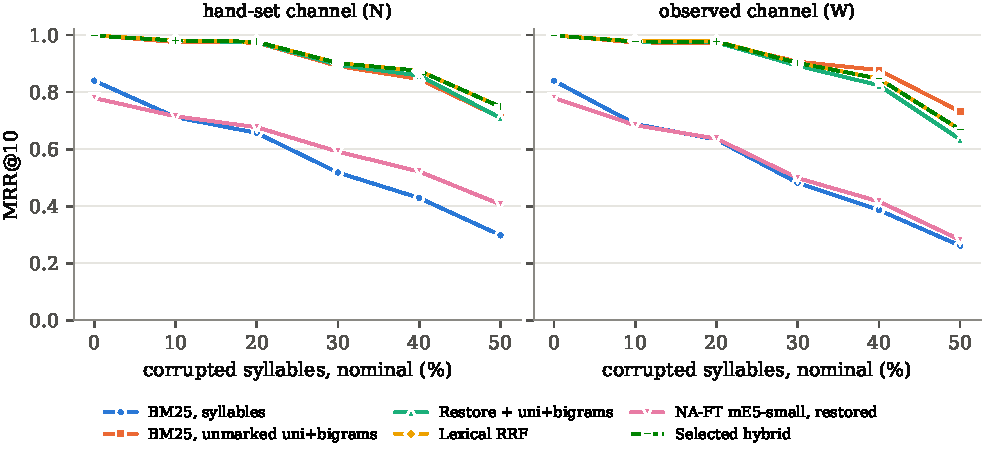
\includegraphics[width=0.6\linewidth]{generated/fig_noise.pdf}
\caption{\mrr{} on the noise sweep: the same test fragments with 0--50\% of their syllables corrupted by
the noise channel.}
\label{fig:noise}
\end{figure}

\begin{table*}[t]
\centering
\caption{MRR@10 on the noise sweep: the same 1241 test fragments with a growing share of
corrupted syllables, under the hand-set channel (N), the channel sampled from the variation observed between
transcriptions (W) and the hand-set operations re-weighted by the observed shares (E, 50\% only;
Section~\ref{sec:validity}). Columns give the nominal rate; the realised share of changed syllables is in the
last row. NA-FT: mean over three seeds.}
\label{tab:noise}
\footnotesize
\setlength{\tabcolsep}{3.4pt}
\begin{tabular}{@{}lrrrrrrrrrrrr@{}}
\toprule
 & & \multicolumn{5}{c}{hand-set channel (N)} & \multicolumn{5}{c}{observed channel (W)} & \multicolumn{1}{c}{E} \\
\cmidrule(lr){3-7} \cmidrule(lr){8-12}
System & 0\% & 10\% & 20\% & 30\% & 40\% & 50\% & 10\% & 20\% & 30\% & 40\% & 50\% & 50\% \\
\midrule
BM25, syllables & 0.840 & 0.712 & 0.657 & 0.518 & 0.429 & 0.298 & 0.688 & 0.634 & 0.481 & 0.386 & 0.261 & 0.315 \\
BM25, unmarked uni+bigrams & 1.000 & 0.975 & 0.974 & 0.891 & 0.846 & 0.711 & 0.974 & 0.973 & 0.907 & 0.877 & 0.732 & 0.728 \\
BM25, char.\ 3-grams in syllables & 0.616 & 0.396 & 0.307 & 0.218 & 0.151 & 0.118 & 0.459 & 0.394 & 0.283 & 0.218 & 0.155 & 0.113 \\
BM25, char.\ 5-grams across syllables & 0.989 & 0.965 & 0.968 & 0.916 & 0.907 & 0.844 & 0.942 & 0.930 & 0.856 & 0.829 & 0.673 & 0.857 \\
BM25, sound-alike key & 0.999 & 0.988 & 0.987 & 0.943 & 0.931 & 0.867 & 0.979 & 0.974 & 0.887 & 0.832 & 0.633 & 0.825 \\
Restore + uni+bigrams & 0.999 & 0.981 & 0.975 & 0.896 & 0.858 & 0.709 & 0.977 & 0.974 & 0.893 & 0.824 & 0.634 & 0.713 \\
Lexical RRF & 0.999 & 0.981 & 0.977 & 0.902 & 0.875 & 0.749 & 0.978 & 0.978 & 0.903 & 0.847 & 0.668 & 0.748 \\
NA-FT mE5-small, restored & 0.779 & 0.715 & 0.677 & 0.591 & 0.522 & 0.407 & 0.684 & 0.637 & 0.499 & 0.416 & 0.282 & 0.414 \\
Selected hybrid & 0.998 & 0.981 & 0.977 & 0.902 & 0.875 & 0.749 & 0.978 & 0.977 & 0.902 & 0.847 & 0.668 & 0.748 \\
\midrule
realised (\%) & 0 & 13 & 19 & 31 & 40 & 50 & 13 & 19 & 31 & 40 & 50 & 50 \\
\bottomrule
\end{tabular}
\end{table*}


\subsection{Query-type classification}\label{sec:res_qtype}
Logistic regression predicts the query type with \QtypeAccLR\% accuracy (macro-F1 \QtypeMacroFLR), Naive
Bayes with \QtypeAccNB\% (macro-F1 \QtypeMacroFNB; Table~\ref{tab:qtype}). Unmarked fragments and
descriptions are almost always recognised (recall \QtypeRecallTwo\% and \QtypeRecallFive\%). Noisy fragments
are confused with exact ones (recall \QtypeRecallThree\%) when the noise produces valid syllables, for
instance \vi{sương}$\rightarrow$\vi{xương}. Paraphrases remain hard (recall \QtypeRecallFour\%): the
classifier has only \QtypeTrainFour{} training examples of them, and a paraphrase looks like a lyric line.
Class weighting raises this recall from \QtypeRecallFourPlain\% and the accuracy from \QtypeAccLRPlain\%. For
the same reason unmarked paraphrases are often taken for unmarked fragments (recall \QtypeRecallFourU\%),
while unmarked descriptions are recognised (\QtypeRecallFiveU\%). Confusing a paraphrase with a fragment
matters because the hybrid gives the two types different weights (Section~\ref{sec:res_hybrid}), and it is
the main cause of the paraphrases that the hybrid misses (Section~\ref{sec:res_errors}).

\begin{table}[t]
\centering
\caption{Confusion matrix of the query-type classifier (logistic regression) on the test queries. Rows: true type;
columns: predicted type. Accuracy 89.4\%
(Naive Bayes: 74.6\%). Q4u and Q5u are Q4 and Q5 typed without marks.}
\label{tab:qtype}
\small
\begin{tabular}{@{}lrrrrrrrr@{}}
\toprule
 & \multicolumn{7}{c}{predicted} & \\
\cmidrule(lr){2-8}
true & Q1 & Q2 & Q3 & Q4 & Q5 & Q4u & Q5u & recall \\
\midrule
Q1 & 1208 & 10 & 14 & 9 & 0 & 0 & 0 & 97\% \\
Q2 & 7 & 1224 & 0 & 0 & 0 & 10 & 0 & 99\% \\
Q3 & 224 & 9 & 1006 & 2 & 0 & 0 & 0 & 81\% \\
Q4 & 83 & 0 & 1 & 124 & 19 & 0 & 0 & 55\% \\
Q5 & 0 & 0 & 0 & 4 & 223 & 0 & 0 & 98\% \\
Q4u & 0 & 70 & 0 & 0 & 0 & 133 & 24 & 59\% \\
Q5u & 0 & 0 & 0 & 0 & 0 & 3 & 224 & 99\% \\
\bottomrule
\end{tabular}
\end{table}


\subsection{Dense retrieval and noise-aware fine-tuning}\label{sec:res_dense}

\begin{table*}[t]
\centering
\caption{Dense, fine-tuned, hybrid and reranked retrieval on the test split (MRR@10). Every choice of model or weights was made on the dev split.}
\label{tab:neural}
\footnotesize
\setlength{\tabcolsep}{3.3pt}
\begin{tabular}{@{}l rrrrr r rrr@{}}
\toprule
 & \multicolumn{5}{c}{MRR@10 by query type} & & \multicolumn{3}{c}{macro average} \\
\cmidrule(lr){2-6} \cmidrule(l){8-10}
System & Q1 & Q2 & Q3 & Q4 & Q5 & Macro & S@1 & S@10 & R@100 \\
 \scriptsize{queries} & \scriptsize{1241} & \scriptsize{1241} & \scriptsize{1241} & \scriptsize{227} & \scriptsize{227} & & & & \\
\midrule
\multicolumn{10}{l}{\textit{Reference}} \\
\quad RRF, weights tuned on dev & 0.999 & 0.995 & 0.943 & 0.344 & 0.930 & 0.842 & 0.820 & 0.886 & 0.945 \\
\addlinespace
\multicolumn{10}{l}{\textit{Dense, zero-shot (MaxP over 4-line passages)}} \\
\quad mE5-small & \multicolumn{9}{c}{\pending{not run yet}} \\
\quad \quad on restored queries & \multicolumn{9}{c}{\pending{not run yet}} \\
\quad mE5-base & \multicolumn{9}{c}{\pending{not run yet}} \\
\quad \quad on restored queries & \multicolumn{9}{c}{\pending{not run yet}} \\
\quad Vietnamese\_Embedding & \multicolumn{9}{c}{\pending{not run yet}} \\
\quad \quad on restored queries & \multicolumn{9}{c}{\pending{not run yet}} \\
\quad BGE-M3 & \multicolumn{9}{c}{\pending{not run yet}} \\
\quad \quad on restored queries & \multicolumn{9}{c}{\pending{not run yet}} \\
\quad bkai bi-encoder & \multicolumn{9}{c}{\pending{not run yet}} \\
\quad \quad on restored queries & \multicolumn{9}{c}{\pending{not run yet}} \\
\addlinespace
\multicolumn{10}{l}{\textit{Noise-aware fine-tuning (NA-FT)}} \\
\quad NA-FT mE5-base (3 seeds) & 0.778$^{\ddagger}$ & 0.088$^{\ddagger}$ & 0.646$^{\ddagger}$ & \textbf{0.702}$^{\dagger}$ & 0.639$^{\ddagger}$ & 0.571 & 0.516 & 0.691 & 0.818 \\
\quad \quad on restored queries (3 seeds) & 0.776$^{\ddagger}$ & 0.764$^{\ddagger}$ & 0.644$^{\ddagger}$ & 0.697$^{\dagger}$ & 0.646$^{\ddagger}$ & 0.705 & 0.646 & 0.831 & 0.937 \\
\quad NA-FT mE5-small (3 seeds) & 0.782$^{\ddagger}$ & 0.121$^{\ddagger}$ & 0.628$^{\ddagger}$ & 0.551$^{\dagger}$ & 0.623$^{\ddagger}$ & 0.541 & 0.480 & 0.668 & 0.813 \\
\quad \quad on restored queries (3 seeds) & 0.779$^{\ddagger}$ & 0.768$^{\ddagger}$ & 0.628$^{\ddagger}$ & 0.540$^{\dagger}$ & 0.618$^{\ddagger}$ & 0.667 & 0.600 & 0.803 & 0.925 \\
\quad \quad without noise (seed 1) & 0.795$^{\ddagger}$ & 0.027$^{\ddagger}$ & 0.541$^{\ddagger}$ & 0.674$^{\dagger}$ & 0.700$^{\ddagger}$ & 0.547 & 0.493 & 0.658 & 0.760 \\
\quad \quad without hard negatives (seed 1) & 0.782$^{\ddagger}$ & 0.092$^{\ddagger}$ & 0.658$^{\ddagger}$ & 0.686$^{\dagger}$ & 0.672$^{\ddagger}$ & 0.578 & 0.524 & 0.699 & 0.827 \\
\quad \quad without noise (seed 1) & 0.792$^{\ddagger}$ & 0.056$^{\ddagger}$ & 0.568$^{\ddagger}$ & 0.542$^{\dagger}$ & 0.640$^{\ddagger}$ & 0.520 & 0.462 & 0.639 & 0.763 \\
\quad \quad without hard negatives (seed 1) & 0.779$^{\ddagger}$ & 0.130$^{\ddagger}$ & 0.635$^{\ddagger}$ & 0.551$^{\dagger}$ & 0.614$^{\ddagger}$ & 0.542 & 0.479 & 0.671 & 0.816 \\
\addlinespace
\multicolumn{10}{l}{\textit{Hybrid: lexical lists + NA-FT mE5-base (seed 3), restored queries}} \\
\quad RRF, equal weights & 0.859$^{\ddagger}$ & 0.862$^{\ddagger}$ & 0.790$^{\ddagger}$ & 0.434$^{\dagger}$ & 0.906 & 0.770 & 0.689 & 0.904 & 0.978 \\
\quad RRF, weights tuned on dev & \textbf{0.999} & \textbf{0.995} & \textbf{0.943} & 0.344 & \textbf{0.930} & 0.842 & 0.820 & 0.886 & 0.945 \\
\quad RRF, weights per predicted type & 0.998 & \textbf{0.995} & \textbf{0.943} & 0.532$^{\dagger}$ & 0.928 & \textbf{0.879} & 0.851 & 0.923 & 0.965 \\
\quad RRF, weights per true type (oracle) & 0.999 & 0.995 & 0.943 & 0.674$^{\dagger}$ & 0.930 & 0.908 & 0.877 & 0.959 & 0.987 \\
\addlinespace
\multicolumn{10}{l}{\textit{Cross-encoder reranking of the top 20 of the selected hybrid}} \\
\quad first stage, same queries & 0.993 & 0.996 & 0.949 & 0.532$^{\dagger}$ & 0.928 & 0.880 & 0.852 & 0.924 & 0.964 \\
\quad bge-reranker-v2-m3 & 0.971$^{\ddagger}$ & 0.977$^{\ddagger}$ & 0.957 & 0.682$^{\dagger}$ & 0.895 & 0.896 & 0.870 & 0.931 & 0.964 \\
\quad Vietnamese\_Reranker & 0.945$^{\ddagger}$ & 0.943$^{\ddagger}$ & 0.914 & 0.650$^{\dagger}$ & 0.789$^{\ddagger}$ & 0.848 & 0.796 & 0.931 & 0.964 \\
\bottomrule
\end{tabular}

\vspace{2pt}
\parbox{\textwidth}{\footnotesize $\dagger$/$\ddagger$: significantly better/worse than the reference lexical system (RRF, weights tuned on dev; paired randomization test, Holm correction within each column, $p<0.05$). Bold: best value per column among runs over every query, oracle rows excluded. NA-FT rows average the per-query scores of the seeds before testing. Reranking rows are evaluated on the queries that were reranked.}
\end{table*}


\paragraph{Zero-shot bi-encoders handle paraphrases, not missing marks.} Without fine-tuning, mE5-base is the
best dense model (macro \MDenseEbaseRestMacro{} on restored queries, Table~\ref{tab:neural}). It is the best
of all systems on paraphrases (\MDenseEbaseFour, against \BestLexQfour{} for the best lexical model), but far
below lexical retrieval on fragments (\MDenseEbaseOne{} on \Qone) and on descriptions (\MDenseEbaseFive,
against \MLyrMetaFive{} for BM25 with metadata): a description is about the whole song, and a passage of four
lines rarely contains what it describes. The bkai bi-encoder, trained on segmented prose, is the weakest
model (macro \MDenseBkaiMacro). All three collapse on unmarked fragments (mE5-base: \MDenseEbaseTwo{} on
\Qtwo): for these encoders an unmarked query is a different string from its marked passage. Restoring the
marks before encoding repairs this (\MDenseEbaseRestTwo{} for mE5-base) and changes no other type
(Table~\ref{tab:planned}, first row), so every hybrid uses restored queries.

\paragraph{Noise-aware fine-tuning helps where lexical retrieval is already strong.} NA-FT raises mE5-small
from \MDenseEsmallRestMacro{} to \MNaftRestMacro{} macro \mrr{} on restored queries (mean of three seeds;
per-seed macro from \NaftRestSeedMin{} to \NaftRestSeedMax, standard deviation \NaftRestSeedSd). The gain is
significant on every fragment type and largest on noisy fragments (\PlNaftThree) and at 50\% noise
(\PlNaftNFifty); paraphrases gain \PlNaftFour, and descriptions lose \PlNaftFive{} (not significant), as no
training pair resembles a description. The fine-tuned small model is still worse than zero-shot mE5-base on
paraphrases (\MNaftRestFour{} against \MDenseEbaseRestFour) and descriptions. The ablations credit the noise
with the gains: trained on clean pairs, seed~1 loses \PlNonoiseThree{} on noisy fragments and \PlNonoiseTwo{}
on unmarked ones, and gains \PlNonoiseFive{} on descriptions, whereas random negatives in place of
BM25-mined hard negatives change no type significantly (at most \PlRandnegFour, on paraphrases). Training on
unmarked queries is no substitute for restoration: NA-FT saw unmarked fragments in training but reaches only
\MNaftTwo{} on \Qtwo{} as typed, against \MNaftRestTwo{} on restored queries.

\subsection{Hybrid retrieval and reranking}\label{sec:res_hybrid}

\begin{table}[t]
\centering
\caption{One weight $w$ for the dense list for every query: hybrid of the lexical lists (weights fixed at their tuned
values) and NA-FT mE5-small (seed 3) on restored queries, MRR@10 on the test split. The $w$ that maximises the macro average on the
development split is 0.25. Last row: $w=8$ for queries predicted
as Q4 and Q4u, $w=0$ otherwise.}
\label{tab:dense_weight}
\small
\setlength{\tabcolsep}{4.5pt}
\begin{tabular}{@{}l rrrrrr r@{}}
\toprule
$w$ & Q1 & Q2 & Q3 & Q4 & Q5 & Q4u & Macro \\
\midrule
0 & 0.999 & 0.995 & 0.943 & 0.344 & 0.930 & 0.299 & 0.842 \\
0.25 & 0.980 & 0.979 & 0.934 & 0.402 & 0.876 & 0.378 & 0.834 \\
0.5 & 0.968 & 0.968 & 0.916 & 0.435 & 0.852 & 0.416 & 0.828 \\
1 & 0.951 & 0.948 & 0.889 & 0.462 & 0.812 & 0.436 & 0.812 \\
2 & 0.933 & 0.929 & 0.857 & 0.477 & 0.757 & 0.448 & 0.791 \\
4 & 0.913 & 0.907 & 0.819 & 0.510 & 0.715 & 0.471 & 0.773 \\
8 & 0.891 & 0.883 & 0.787 & 0.525 & 0.679 & 0.488 & 0.753 \\
\midrule
per predicted type & 0.999 & 0.995 & 0.943 & 0.458 & 0.930 & 0.415 & 0.865 \\
\bottomrule
\end{tabular}
\end{table}


\paragraph{A dense list helps only with weights per query type.} Table~\ref{tab:dense_weight} adds the dense
list of the selected hybrid (NA-FT mE5-small, seed~3, the best seed on development queries) to the tuned
lexical fusion with one weight $w$ for every query. Every weight that helps paraphrases costs more on the
other types: at $w=8$ paraphrases reach \DwEightFour, but noisy fragments fall to \DwEightThree{} and
descriptions to \DwEightFive. The single weight with the best development macro, $w=\DwMacroTunedW$, gains on
paraphrases (\DwQuarterFour{} against \DwZeroFour) but loses more on descriptions (\DwQuarterFive{} against
\DwZeroFive) and fragments, and the test macro falls from \DwZeroMacro{} to \DwQuarterMacro; tuned on all
development queries pooled, as in our global fusion, the weight is 0, and the hybrid with global weights is
the lexical fusion (Table~\ref{tab:neural}). With weights per type, the cross-validation guard gives the dense
list a weight of \DwAdaptiveWeight{} for queries predicted as \DwAdaptiveTypes{} and none elsewhere.
Paraphrases then rise from \PlHybridFourA{} to \PlHybridFourB{} while no other type changes
(Table~\ref{tab:planned}), and macro \mrr{} rises from \MFuseGlobalMacro{} to \MHybNaftAdaptiveMacro. The
classifier limits the gain: with the true query type, paraphrases reach \PlOracleFourB{} (\PlOracleFour). A
weight of 8, the largest of the grid, lets the dense model decide the ranking of a predicted paraphrase:
any song in its top 100 outscores a song that both bigram lists rank first but the dense list misses
($8/160 > 2.5/61$), and the lexical lists only break ties.

\paragraph{Which dense model.} On the development split the hybrids with NA-FT mE5-small and with zero-shot
mE5-base are tied (macro \MHybNaftAdaptiveDev{} and \MHybEbaseAdaptiveDev); on the test split mE5-base is
better on paraphrases (\PlOtherdenseFourB{} against \PlOtherdenseFourA), as it is on its own, and the two
are equal elsewhere. Fine-tuning on fragments improved the dense model where the hybrid does not need it.

\paragraph{Reranking.} The cross-encoder reranks the top \RerankDepth{} songs of the selected hybrid for a
stratified sample of \RerankQueries{} test queries (40 of each type, unmarked types included). On paraphrases
it adds \PlRerankFour{} (\PlRerankFourA{} to \PlRerankFourB, significant even on 40 queries), but it loses on
every other type, from \PlRerankTwo{} on unmarked fragments to \PlRerankFive{} on descriptions (none
significant on 40 queries), and the macro average falls from \MFirstSampleMacro{} to \MRerankMacro. Scoring a
single passage per song, the cross-encoder judges meaning, which suits paraphrases, but it ignores the exact
word sequence that the first stage matches in a fragment and the rest of the song that a description is
about. Reranking would therefore pay off only for queries predicted as paraphrases, and at
\RerankSecPerQuery{} s per query on our CPU it is by far the most expensive component
(Section~\ref{sec:res_efficiency}).

\begin{table*}[t]
\centering
\caption{Planned comparisons on the test split: change in MRR@10 from system A to system B (B $-$ A), per query
type and at 50\% noise. $^{*}$: $p<0.05$, two-sided paired randomization test with 10{,}000 permutations, Holm
correction over the 8 comparisons within each column. Systems with three seeds enter with their mean per
query. Macro: change of the macro average, not tested. Reranking was run on 40 sampled queries per type.}
\label{tab:planned}
\footnotesize
\setlength{\tabcolsep}{4pt}
\begin{tabular}{@{}l rrrrr r r@{}}
\toprule
Comparison (A $\rightarrow$ B) & Q1 & Q2 & Q3 & Q4 & Q5 & N50 & Macro \\
\midrule
mE5-base: queries as typed $\rightarrow$ restored & 0.000 & \ensuremath{+}0.667$^{*}$ & \ensuremath{+}0.001 & \ensuremath{-}0.001 & \ensuremath{+}0.001 & \ensuremath{+}0.008 & \ensuremath{+}0.133 \\
mE5-small, restored: zero-shot $\rightarrow$ NA-FT & \ensuremath{+}0.088$^{*}$ & \ensuremath{+}0.091$^{*}$ & \ensuremath{+}0.147$^{*}$ & \ensuremath{+}0.080$^{*}$ & \ensuremath{-}0.043 & \ensuremath{+}0.140$^{*}$ & \ensuremath{+}0.073 \\
NA-FT (seed 1) $\rightarrow$ without noise & \ensuremath{-}0.035$^{*}$ & \ensuremath{-}0.085$^{*}$ & \ensuremath{-}0.125$^{*}$ & \ensuremath{+}0.012 & \ensuremath{+}0.059$^{*}$ & \ensuremath{-}0.172$^{*}$ & \ensuremath{-}0.035 \\
NA-FT (seed 1) $\rightarrow$ random negatives & \ensuremath{+}0.004 & \ensuremath{-}0.003 & \ensuremath{+}0.005 & \ensuremath{+}0.011 & \ensuremath{-}0.004 & \ensuremath{+}0.008 & \ensuremath{+}0.002 \\
Lexical fusion $\rightarrow$ hybrid & 0.000 & 0.000 & 0.000 & \ensuremath{+}0.114$^{*}$ & 0.000 & 0.000 & \ensuremath{+}0.023 \\
Hybrid: predicted $\rightarrow$ true query type & 0.000 & 0.000 & 0.000 & \ensuremath{+}0.067$^{*}$ & 0.000 & 0.000 & \ensuremath{+}0.013 \\
Hybrid: NA-FT mE5-small $\rightarrow$ mE5-base & \ensuremath{-}0.002 & \ensuremath{-}0.001 & 0.000 & \ensuremath{+}0.038$^{*}$ & \ensuremath{-}0.002 & 0.000 & \ensuremath{+}0.006 \\
Hybrid $\rightarrow$ cross-encoder reranking & \ensuremath{-}0.042 & \ensuremath{-}0.025 & \ensuremath{-}0.032 & \ensuremath{+}0.104$^{*}$ & \ensuremath{-}0.080 & -- & \ensuremath{-}0.015 \\
\bottomrule
\end{tabular}
\end{table*}


\subsection{Validity of the synthetic queries}\label{sec:res_validity}
\maybeinput{generated/tab_channel}
The \RealPairs{} pairs of versions align \RealAligned{} syllables, of which \RealSubs{} are substituted
(\RealSubsPerK{} per thousand); \RealOtherWordShare\% of the substitutions are different words, which only
\Qfour{} imitates. Among the \RealChanN{} substitutions of the kinds the channel models
(Table~\ref{tab:channel}), tone changes (\RealChanTone\%) and typing differences (\RealChanTypo\%) are more
frequent than the hand-set weights assume, and final consonants much rarer (\RealChanFinal\% against
\DefWFinal\%). Only \RealKnownInitialShare\% of the initial changes are the dialectal mergers of the channel;
the others keep the rhyme and change the word (\vi{muộn/buồn}, \vi{nồng/mộng}), as misheard lyrics do.
The real transcriptions thus contain more tone and typing differences and fewer coda changes than the
channel assumes, but repeating the sweep with the estimated weights changes little (last column of
Table~\ref{tab:noise}): over the \NoiseSystems{} systems and the five noise levels, \mrr{} changes by
\ChanDiffMean{} on average and by at most \ChanDiffMaxAbs, and the orderings of the systems at equal rates
agree closely (Kendall's $\tau$ \TauChannelMean{} on average, at least \TauChannelMin). The conclusions about
noise do not depend on the hand-set weights.

\maybeinput{generated/tab_validity}
\paragraph{Agreement between query types.} The rule-based types order the \ValSystems{} systems much like the
macro average of the other types (Table~\ref{tab:validity}; $\tau$ from \TauLooQone{} for exact fragments to
\TauLooQthree{} for noisy ones), and so do descriptions (\TauLooQfive). The ordering on clean fragments
survives heavy noise ($\tau$ \TauNoiseFifty{} between 0\% and 50\%). Paraphrases are the exception: their
ordering is unrelated to that of the other types ($\tau$ \TauLooQfour), and the lowest agreement of any two
types is between exact fragments and paraphrases ($\tau$ \TauPairMin). This follows from the results rather
than from a flaw of the generator: dense models are the worst systems on fragments and the best on
paraphrases, so a collection would rank systems very differently depending on which kind of query it holds.
The rule-based and LLM-written families agree moderately ($\tau$ \TauFamily). A collection that leaves out
paraphrases, or has only paraphrases, would reach different conclusions about dense retrieval.

\paragraph{Discriminative power.} Every type separates most of the \DPPairs{} pairs of systems at
$\alpha=0.05$ (\DPMin--\DPMax\% for the main types, \DPQfourU\% for unmarked paraphrases). The \NLLMClustersTest{}
paraphrases and descriptions separate systems almost as often as the \NSweepFragments{} fragments of each
rule-based type, partly because many systems tie at the ceiling on fragments.

\subsection{Error analysis}\label{sec:res_errors}
We examined the test queries that the selected hybrid misses (target below rank 10). It misses
\ErrQoneFail{} exact and \ErrQtwoFail{} unmarked fragments.

\paragraph{Noisy fragments} fail \ErrQthreeFail{} times out of \ErrQthreeN. The failures are short
(\ErrQthreeLenFail{} syllables against \ErrQthreeLenOk{} for the others), and the noise leaves them few
syllables of the lyrics (\ErrQthreeOverlapFail{} of their unmarked syllables occur in the target, against
\ErrQthreeOverlapOk) and short intact runs (\ErrQthreeRunFail{} against \ErrQthreeRunOk{} syllables). In
\vi{bao gnày nghe tiến mưa}, from \vi{bao ngày nghe tiếng mưa} (\gloss{so many days hearing the rain}), a
transposition and a coda merger leave three common syllables, which occur together in many songs.

\paragraph{Paraphrases} fail \ErrQfourFail{} times out of \ErrQfourN. The classifier took \ErrQfourPredQone{}
of these for exact fragments and \ErrQfourPredQfive{} for descriptions, so the dense list got no weight; only
\ErrQfourPredQfour{} were recognised and still missed. Missed paraphrases are shorter (\ErrQfourLenFail{}
against \ErrQfourLenOk{} syllables) and share fewer syllables with the lyrics (\ErrQfourOverlapFail{} against
\ErrQfourOverlapOk): the more freely a paraphrase is worded, the more it reads like the common language of
love songs. Medleys, which hold the lines of several songs, rank first for \ErrQfourMedleyFail\% of the missed
paraphrases and \ErrQfourMedleyOk\% of the others, so they are not a main source of error.

\paragraph{Descriptions} fail \ErrQfiveFail{} times. They quote the lyrics less than the descriptions that
succeed (overlap \ErrQfiveOverlapFail{} against \ErrQfiveOverlapOk; longest copied run \ErrQfiveRunFail{}
against \ErrQfiveRunOk{} syllables) and describe the song in general terms. \ErrQfiveArtistFailN{} of them
name the singer or composer, but the tuned fusion gives the metadata list no weight, and \vi{bài vui tươi của
sơn tùng về lần đầu rung động\dots} (\gloss{a cheerful song by Sơn Tùng about falling in love for the first
time\dots}) ranks another song by the same singer above the target. A metadata weight for queries predicted
as descriptions is an obvious refinement.

\subsection{Effect of catalogue size}\label{sec:res_catalogue}
\begin{table*}[t]
\centering
\caption{MRR@10 on the test split when the index keeps a random share of the 6213 clusters (the target
cluster is always kept; mean over 5 random draws). Rankings are those of the full index restricted to the
kept songs; the hybrid is fused again from the restricted lists.}
\label{tab:catalogue}
\scriptsize
\setlength{\tabcolsep}{3.2pt}
\begin{tabular}{@{}l rrr rrr rrr rrr@{}}
\toprule
 & \multicolumn{3}{c}{Q1} & \multicolumn{3}{c}{Q4} & \multicolumn{3}{c}{Q5} & \multicolumn{3}{c}{Macro} \\
\cmidrule(lr){2-4} \cmidrule(lr){5-7} \cmidrule(lr){8-10} \cmidrule(lr){11-13}
Share kept & 25\% & 50\% & 100\% & 25\% & 50\% & 100\% & 25\% & 50\% & 100\% & 25\% & 50\% & 100\% \\
\midrule
BM25, syllables & 0.912 & 0.877 & 0.840 & 0.440 & 0.383 & 0.325 & 0.868 & 0.834 & 0.802 & 0.604 & 0.561 & 0.521 \\
BM25, unmarked bigrams & 1.000 & 1.000 & 1.000 & 0.399 & 0.347 & 0.288 & 0.934 & 0.918 & 0.898 & 0.857 & 0.841 & 0.821 \\
Restore + bigrams & 1.000 & 0.999 & 0.999 & 0.459 & 0.401 & 0.342 & 0.956 & 0.945 & 0.932 & 0.876 & 0.859 & 0.840 \\
Lexical RRF & 1.000 & 0.999 & 0.999 & 0.459 & 0.399 & 0.344 & 0.954 & 0.944 & 0.930 & 0.877 & 0.859 & 0.842 \\
mE5-base, restored & 0.788 & 0.750 & 0.711 & 0.707 & 0.653 & 0.597 & 0.756 & 0.704 & 0.642 & 0.729 & 0.684 & 0.634 \\
NA-FT (seed 1), restored & 0.879 & 0.850 & 0.819 & 0.639 & 0.588 & 0.536 & 0.652 & 0.602 & 0.544 & 0.758 & 0.719 & 0.675 \\
Selected hybrid & 1.000 & 0.999 & 0.999 & 0.567 & 0.515 & 0.458 & 0.955 & 0.944 & 0.930 & 0.898 & 0.883 & 0.865 \\
\bottomrule
\end{tabular}
\end{table*}

Our catalogue is small next to a commercial service. To see how the results depend on its size, we shrink it:
the index keeps a random share of the other clusters (the target cluster always stays), and each ranking is
restricted to the kept songs (Table~\ref{tab:catalogue}). The restricted rankings keep the term statistics of
the full index, a small advantage for BM25 in the smaller catalogues. Exact fragments are unaffected for bigram
indexes (the hybrid reaches \CatHybNaftAdaptiveOneQuarter{} on a quarter of the catalogue and
\CatHybNaftAdaptiveOneFull{} on all of it), whereas unigrams lose \CatSylOneDrop{} per doubling of the
catalogue. Paraphrases are the most sensitive: each doubling costs the hybrid about
\CatHybNaftAdaptiveFourDrop{} on \Qfour{} (\CatHybNaftAdaptiveFourQuarter{} on a quarter,
\CatHybNaftAdaptiveFourFull{} on the full catalogue), and mE5-base alone loses as much
(\CatDenseEbaseRestFourDrop{} per doubling). Descriptions lose \CatHybNaftAdaptiveFiveDrop{} per doubling. In
a catalogue many times larger, fragments would thus remain largely solved while the gap to paraphrases would
widen, and our results on paraphrases and descriptions are best read as upper bounds for larger catalogues.

\subsection{Efficiency}\label{sec:res_efficiency}
\begin{table}[t]
\centering
\caption{Cost on four CPU cores without a GPU. Index: encoding the 79,328
passages (dense) or building the inverted index (lexical), and the size of the passage vectors. Query: encoding one
query; search: exact search for one query (ms). mE5-small and NA-FT mE5-small share one architecture; their difference
shows the variation between timing runs.}
\label{tab:efficiency}
\small
\setlength{\tabcolsep}{4pt}
\begin{tabular}{@{}l r r r r r@{}}
\toprule
 & Passages/s & Index & MB & Query (ms) & Search (ms) \\
\midrule
mE5-small & 83 & 16 min & 122 & 6 & 5 \\
NA-FT mE5-small & 99 & 13 min & 122 & 5 & 5 \\
mE5-base & 28 & 47 min & 244 & 15 & 9 \\
bkai bi-encoder & 29 & 45 min & 244 & 14 & 8 \\
\midrule
BM25, syllable uni+bigrams & -- & 3 s & -- & -- & 0.3 \\
BM25, unmarked uni+bigrams & -- & 4 s & -- & -- & 0.4 \\
Diacritic restoration & -- & -- & -- & 0.6 & -- \\
bge-reranker-v2-m3, top 20 & -- & -- & -- & -- & 100 \\
\bottomrule
\end{tabular}
\end{table}

Table~\ref{tab:efficiency} gives the costs on our machine. Lexical search takes well under a millisecond per
query (\EffLexMsNodiac{} ms for unmarked uni+bigrams) and an index is built in seconds; restoration adds
\RestoreMsAll{} ms per query. A dense model encodes the \NPassages{} passages once in \EffEncodeMinNaftesmalls{}
(NA-FT mE5-small) to \EffEncodeMinEbase{} minutes (mE5-base), a query in \EffQueryMsNaftesmalls{} to
\EffQueryMsEbase{} ms, and exact search over the passage vectors takes \EffSearchMsNaftesmalls{} to
\EffSearchMsEbase{} ms. Training NA-FT takes about \NaftTrainMinutes{} minutes per model. The selected hybrid
therefore answers a query in about \EffHybridMs{} ms on four CPU cores without a GPU, whereas the cross-encoder
needs \RerankSecPerQuery{} s to rerank \RerankDepth{} songs.

%=====================================================================
\section{Discussion and limitations}\label{sec:limitations}
%=====================================================================

\paragraph{What the results suggest for Vietnamese song search.} Index syllable bigrams over unmarked text,
or restore the marks of a query and search marked bigrams; do not rely on character $n$-grams for tolerance
to typing errors; restore marks before any dense encoder; and give a dense model weight only for queries that
look like paraphrases. The gain then depends on recognising paraphrases, which our classifier does for about
half of them; a classifier trained on more varied paraphrases, or probabilities instead of a hard decision,
are the natural next steps. NA-FT, which needs no LLM and trains in about \NaftTrainMinutes{} minutes on a CPU, is worth its cost for a
dense-only engine, not for a hybrid.

\paragraph{Catalogue size and source.} The catalogue has \NSongs{} songs, \UniformShare\% of them a uniform sample
of one chord site, so songs that nobody has transcribed for guitar are missing, and a commercial service holds
far more songs. We stopped the crawl at \CrawlSongs{} songs and did not add distractor songs, so the effect of
a larger catalogue is extrapolated from smaller ones: Section~\ref{sec:res_catalogue} shows that exact and
unmarked fragments are robust to the size of the catalogue while paraphrases and descriptions are not.

\paragraph{Synthetic queries.} Fragments are cut from the lyrics, which favours lexical models, and the
ambiguity filter removes fragments shared by two songs, which may remove some of the lines people remember
best. Paraphrases and descriptions written by an LLM may differ from people's in vocabulary and style. All of
them come from one model family; the prompt and writer variants (Q4s, Q5g) show how far the conclusions
depend on the prompt and on what the writer saw, but not what another generator would write. The \Qfive{}
writer saw the lyrics and the artist, which makes these descriptions more precise than those of a person who
heard the song once; Q5g, written from a gist alone, is the more realistic description set.
\Qfouru{} and \Qfiveu{} only remove marks, while people who type without marks may also write shorter or
differently worded queries. Queries written by an LLM can also favour retrieval models that resemble it
\citep{rahmani2024synthetic}; none of our retrieval models is an LLM, but the bi-encoders were trained on
similar web text. The checks of Section~\ref{sec:validity} show whether conclusions depend on the query type,
the prompt or the channel, but not whether people search the same way; real queries, for instance from the
logs of a music service or from a questionnaire, would show that.

\paragraph{Noise channel.} The confusion classes of the hand-set channel come from dialectology, but their
probabilities and the weights of the operations were set by hand. The observed channel replaces them with the
kinds of substitution found between transcriptions, but these come from people writing down lyrics they know,
at about one error per hundred syllables; the error rates of people who recall a lyric, and errors such as
abbreviations (\vi{ko} for \vi{không}) and mixed scripts, remain unmodelled. Lexical normalisation corpora of
Vietnamese social media text \citep{nguyen2024vilexnorm} could calibrate the typing part of the channel against
real informal writing.

\paragraph{Models we could not evaluate.} Larger multilingual and Vietnamese encoders (BGE-M3,
Vietnamese\_Embedding), Vietnamese rerankers \citep{dang2025viranker} and neural diacritic restorers
\citep{dang2020tdp} were not available in our computing environment, which had no GPU and, during the revision,
no access to the model repository. Our Kneser--Ney restorer already restores \RestoreAccAll\% of the syllables
of unmarked fragments, so a neural restorer matters mostly for unmarked paraphrases and descriptions. NA-FT has
no paraphrase-like training pairs by design (it uses no LLM); training a bi-encoder on paraphrases is the most
direct way to attack the weakest query type.

\paragraph{Development data.} The method was designed on the pilot catalogue, whose clusters also hold test
queries. Section~\ref{sec:res_nonpilot} shows the results on the other clusters.

\paragraph{Copyright and release.} Lyrics are copyrighted. We release the code that rebuilds the corpus from
the crawled pages, the song identifiers, source URLs, crawl dates and a checksum of each song's normalised
lyrics (so that a re-crawl can be checked against ours), the queries and the run files, but not the lyrics.
Queries are short fragments or paraphrases. The crawler identified itself as a research crawler in its user
agent, fetched one page per second and followed the site's \texttt{robots.txt}. \authornote{check the terms of
the source sites and the journal's data policy}

%=====================================================================
subsection{Results outside the pilot catalogue}\label{sec:res_nonpilot}
These results come from the round-1 analyses that are being rerun; the numbers marked \pending{?} are filled in by that run.

\section{Conclusion}
%=====================================================================
ViSongSearch is a test collection for finding Vietnamese songs from imperfect memories of their lyrics, with
queries that range from exact fragments to paraphrases and descriptions, and with validity checks that need
no participants. Three conclusions stand out. First, the index unit and the handling of diacritics matter
more than the retrieval model: syllable bigrams over unmarked or restored text retrieve exact, unmarked and
noisy fragments almost perfectly and degrade gracefully with noise, whereas character $n$-grams, segmented
words and pseudo-relevance feedback bring little or harm. Second, paraphrases remain the open problem.
Bi-encoders handle them better than lexical models, but only when the diacritics are restored before
encoding, and noise-aware fine-tuning improves a bi-encoder where lexical retrieval is already strong rather
than where it is weak. Third, a dense model improves a hybrid only through weights that depend on the
predicted query type, and the recognition of paraphrases now limits the gain. Better recognition of
paraphrases, use of the metadata for descriptions, larger catalogues and real queries are the next steps.

\section*{Statements}
\paragraph{Data and code availability.} The code that rebuilds the collection from the source pages, the song
identifiers and source URLs, the queries, the run files and the evaluation scripts are available at
\authornote{repository URL}. Lyrics are not redistributed (Section~\ref{sec:limitations}).
\paragraph{Ethics.} The study involves no human participants. The crawled pages are public, and only
song lyrics and metadata were kept; no user accounts or comments were collected.
\paragraph{Use of AI tools.} The code, the experiments and a first draft of this paper were produced with
the help of an AI assistant (Claude, Anthropic), and the \Qfour{} and \Qfive{} queries were written by the same
model (Section~\ref{sec:llm}). Every number in the paper is computed by the released scripts from the run
files. \authornote{the authors checked and take responsibility for the content; add model version if the
venue requires it}

\bibliographystyle{plainnat}
\bibliography{refs}

\appendix
\section{Instructions for LLM-written queries}\label{app:prompts}
Instructions were given in Vietnamese; English translations follow each.

\paragraph{\Qfour{} (paraphrase).}
\vi{Bạn là người nghe nhạc chỉ nhớ mang máng một đoạn lời bài hát tiếng Việt. Đây là đoạn lời thật:
``\{đoạn lời\}''. Hãy viết lại đoạn này như cách bạn nhớ sai: giữ ý chính, nhưng đổi phần lớn từ ngữ (dùng
từ đồng nghĩa, đảo trật tự, bỏ bớt chữ). Không chép nguyên cụm từ 4 chữ trở lên. Viết 1 câu, 8--20 âm
tiết, chữ thường, không dấu câu. Chỉ trả lời câu đó.}

\noindent\emph{You are a listener who only vaguely remembers a fragment of a Vietnamese song. Here is the
real fragment: ``\{fragment\}''. Rewrite it the way you misremember it: keep the main idea but change most
of the words (synonyms, different order, fewer words). Do not copy any phrase of four syllables or more.
Write one sentence of 8--20 syllables, lowercase, without punctuation. Answer with that sentence only.}

\paragraph{\Qfive{} (description).}
\vi{Bạn đang cố tìm một bài hát tiếng Việt nhưng quên tên bài. Thông tin bạn còn nhớ (KHÔNG được nhắc tên
bài): Tên bài (chỉ để bạn biết, cấm viết ra): \{tên\}; Sáng tác: \{nhạc sĩ\}; Ca sĩ: \{ca sĩ\}; Lời bài hát
(một phần): \{lời\}. Hãy viết một câu tìm kiếm như người thật gõ vào Google khi quên tên bài: mô tả nội
dung, cảm xúc, hoàn cảnh, có thể nhớ lờ mờ vài chữ hoặc tên ca sĩ. Không viết tên bài. 1--2 câu, tối đa 35
âm tiết, chữ thường. Chỉ trả lời câu đó.}

\noindent\emph{You are trying to find a Vietnamese song but have forgotten its title. What you remember (do
NOT mention the title): title (for your information only, never write it): \{title\}; composer:
\{composer\}; singers: \{singers\}; part of the lyrics: \{lyrics\}. Write a search query as a real person
would type into Google after forgetting the title: describe the content, feeling or situation; you may
vaguely remember a few words or the singer. Do not write the title. One or two sentences, at most 35
syllables, lowercase. Answer with the query only.}

\noindent For the pilot clusters, whose sources keep a single artist field, the composer and singer lines
were one line, \vi{Tác giả / ca sĩ: \{nghệ sĩ\}}. The filters of Section~\ref{sec:llm} are looser than the
instruction not to copy four syllables: they reject a copied run of five syllables or more for \Qfour.

\paragraph{Q4s (short paraphrase, test only).}
\vi{Bạn là người nghe nhạc chỉ nhớ mang máng một đoạn lời bài hát tiếng Việt. Đây là đoạn lời thật:
``\{đoạn lời\}''. Hãy viết lại đoạn này như cách bạn nhớ sai: giữ ý chính, nhưng đổi phần lớn từ ngữ (dùng
từ đồng nghĩa, đảo trật tự, bỏ bớt chữ). Không chép nguyên cụm từ 4 chữ trở lên. Viết 1 câu ngắn, 5--12 âm
tiết, chữ thường, có dấu tiếng Việt, không dấu câu. Chỉ trả lời câu đó.}

\noindent\emph{As for \Qfour, but: write one short sentence of 5--12 syllables, lowercase, with Vietnamese
marks, without punctuation.}

\paragraph{Gist (first step of Q5g).}
\vi{Đọc lời bài hát dưới đây và tóm tắt nội dung của bài trong 1 câu, tối đa 20 âm tiết: bài nói về ai,
chuyện gì, cảm xúc và hoàn cảnh ra sao. Viết bằng lời của bạn: không dùng lại cụm từ 3 chữ liên tiếp trở lên
của lời bài hát, không trích lời. Chữ thường, có dấu tiếng Việt. \{lời\}}

\noindent\emph{Read the lyrics below and summarise what the song is about in one sentence of at most 20
syllables: who it is about, what happens, the feelings and the situation. Use your own words: do not reuse
any run of three or more consecutive syllables of the lyrics, do not quote. Lowercase, with Vietnamese marks.
\{lyrics\}}

\paragraph{Q5g (description from the gist, test only).}
\vi{Bạn đang cố tìm một bài hát tiếng Việt nhưng quên tên bài và không nhớ lời. Bạn chỉ nhớ bài hát nói
về: ``\{tóm ý\}''. Hãy viết một câu tìm kiếm như người thật gõ vào Google khi quên tên bài: mô tả nội dung,
cảm xúc, hoàn cảnh. 1--2 câu, tối đa 35 âm tiết, chữ thường, có dấu. Chỉ trả lời câu đó.}

\noindent\emph{You are trying to find a Vietnamese song but have forgotten its title and do not remember the
lyrics. You only remember that the song is about: ``\{gist\}''. Write a search query as a real person would
type into Google after forgetting the title: describe the content, feeling or situation. One or two
sentences, at most 35 syllables, lowercase, with marks. Answer with the query only.}

\section{Systems compared in the validity analyses}\label{app:systems}
The agreement and discriminative-power analyses (Table~\ref{tab:validity}) use the following \ValSystems{} runs
over every test query; \NDupRuns{} further runs whose rankings are identical to one of them on every test query
are left out.

\maybeinput{generated/systems_list}

\section{Tuned parameters}\label{app:params}
BM25 ($k_1$, $b$): syllables \KoneSyl, \BSyl; syllable uni+bigrams \KoneSylBi, \BSylBi; words \KoneWord, \BWord;
unmarked syllables \KoneNodiac, \BNodiac; unmarked uni+bigrams \KoneNodiacBi, \BNodiacBi; character 3-grams
\KoneChar, \BChar; character 4-grams across syllables \KoneCharFourX, \BCharFourX; character 5-grams across
syllables \KoneCharFiveX, \BCharFiveX; sound-alike key \KonePhon, \BPhon; metadata \KoneMeta, \BMeta. Query
likelihood: $\mu = \QLmu$. RM3: \RMthreeDocs{} feedback songs, \RMthreeTerms{} terms, original-query weight
\RMthreeOrigW. Metadata weight: $w = \MetaWeight$. Lexical RRF weights (Restore$_{\mathrm{all}}$ uni+bigrams,
unmarked uni+bigrams, character trigrams, metadata): \FuseGlobalWeights. All values were selected on the
development split; the full list is in the released \texttt{results} files.

\ifcoursever
\section{Relation to the SEG301 and TMG301 courses}\label{app:courses}
This appendix belongs to the course submission only and is removed from the journal version. The work is the
joint project of the courses SEG301 (Search Engines) and TMG301 (Text Mining): SEG301 supplies the frame of a
search engine (crawling, indexing, ranking, evaluation), TMG301 the text models inside it. Tables~\ref{tab:seg}
and~\ref{tab:tmg} map each lecture to the part of the work that applies it.

\begin{table}[h]
\centering\small
\caption{SEG301 lectures and where this work applies them.}\label{tab:seg}
\begin{tabular}{@{}p{0.27\linewidth}p{0.55\linewidth}p{0.12\linewidth}@{}}
\toprule
Lecture & Applied as & Where \\
\midrule
1 IR and search engines & known-item song search as the task & \S\ref{sec:qtypes} \\
2 Architecture & crawl, text transformation, index, query processing, ranking, evaluation; web demo & \S\ref{sec:collection}--\ref{sec:methods}, code \\
3 Crawls and feeds & polite resumable crawler (robots.txt, 1 request/s), Unicode clean-up, near-duplicate clusters & \S\ref{sec:corpus}, \S\ref{sec:clusters} \\
4 Processing text & syllable, bigram, word, unmarked and character $n$-gram analysers; vocabulary statistics & \S\ref{sec:lexical} \\
5 Ranking with indexes & sparse inverted index with precomputed BM25 weights, metadata field index & \S\ref{sec:lexical} \\
6 Queries and interfaces & noisy-channel diacritic restoration, Telex decoding, RM3 expansion, result snippets & \S\ref{sec:restoration}, code \\
7 Retrieval models & BM25, query likelihood, relevance model, dense bi-encoders, fine-tuning, cross-encoder & \S\ref{sec:methods} \\
8 Search engine optimisation & song pages with schema.org JSON-LD, sitemap, robots rules, click log (demo) & code (\texttt{app/}) \\
9 Evaluating search engines & test collection, MRR@10, paired randomization test with Holm correction, dev/test discipline, efficiency & \S\ref{sec:setup}, \S\ref{sec:results} \\
10 Classification and clustering & query-type classifier; clusters of song versions & \S\ref{sec:qtype}, \S\ref{sec:clusters} \\
11 Social search & fusion of several result lists (metasearch, RRF) & \S\ref{sec:fusion} \\
12 Beyond bag of words & term dependence through syllable bigrams; one search for all queries vs.\ type-adaptive fusion & \S\ref{sec:lexical}, \S\ref{sec:fusion} \\
\bottomrule
\end{tabular}
\end{table}

\begin{table}[h]
\centering\small
\caption{TMG301 lectures and where this work applies them (lectures 11--15 are not used).}\label{tab:tmg}
\begin{tabular}{@{}p{0.27\linewidth}p{0.55\linewidth}p{0.12\linewidth}@{}}
\toprule
Lecture & Applied as & Where \\
\midrule
01 Regular expressions, normalisation, edit distance & lyric cleaning, NFC and diacritic handling, Damerau--Levenshtein distance of noisy queries & \S\ref{sec:corpus}, \S\ref{sec:noise} \\
02 $n$-gram language models & Kneser--Ney trigram model for diacritic restoration & \S\ref{sec:restoration} \\
03 Naive Bayes & query-type classification & \S\ref{sec:qtype} \\
04 Logistic regression & class-balanced query-type classifier & \S\ref{sec:qtype} \\
05 Vector semantics and embeddings & TF-IDF/BM25 weighting, dense vectors and cosine similarity & \S\ref{sec:lexical}, \S\ref{sec:dense} \\
06 Clustering and text similarity & Jaccard similarity of shingles, MinHash, single-linkage clusters & \S\ref{sec:clusters} \\
07 Transformers and pretrained models & zero-shot bi-encoders and cross-encoder reranking & \S\ref{sec:dense}, \S\ref{sec:rerank} \\
08 Fine-tuning & noise-aware fine-tuning of a bi-encoder & \S\ref{sec:naft} \\
09 Machine translation (related) & diacritic restoration decoded like statistical translation (noisy channel, beam search) & \S\ref{sec:restoration} \\
10 Chatbots and LLMs & LLM-written queries with automatic filters & \S\ref{sec:llm} \\
16 Word senses (related) & most-frequent-form baseline for restoration & \S\ref{sec:restoration} \\
\bottomrule
\end{tabular}
\end{table}
\fi

\end{document}
